% Apresentação da defesa do TCC.
% Visual do modelo institucional 2 do Ifes (docs/slides): os fundos em fundos/
% foram extraídos de modelo2-apresentacao-institucional.odp.
% Compilar com: latexmk -pdf main.tex
\documentclass[aspectratio=169,11pt,t]{beamer}

\usepackage[utf8]{inputenc}
\usepackage[T1]{fontenc}
\usepackage[brazil]{babel}
\usepackage[default]{opensans}
\usepackage[varqu,scaled=0.95]{zi4}
\usepackage{graphicx}
\usepackage{tikz}
\usetikzlibrary{arrows.meta,positioning,calc,shapes.geometric}
\usepackage{listings}
\usepackage{booktabs}

\graphicspath{{figuras/}{fundos/}{../monografia/imagens/}}

% Sem hifenização: em slide, palavra partida atrapalha a leitura
\hyphenpenalty=10000
\exhyphenpenalty=10000

% ---------------------------------------------------------------------------
% Cores do modelo
\definecolor{verdeEsc}{HTML}{006600}  % título da capa
\definecolor{verdeIF}{HTML}{359830}
\definecolor{lima}{HTML}{66CC00}      % subtítulo da capa
\definecolor{vermelho}{HTML}{E83030}  % título dos slides (#FF3333 no modelo)
\definecolor{vermelhoIF}{HTML}{C90C0F}
\definecolor{cinza}{HTML}{555555}     % texto (#666666 no modelo)
\definecolor{cinzaClaro}{HTML}{F2F4F2}

% ---------------------------------------------------------------------------
% Tema: sem navegação, título à esquerda, fundo do modelo
\setbeamertemplate{navigation symbols}{}
\setbeamercolor{normal text}{fg=cinza}
\setbeamercolor{structure}{fg=verdeIF}
\setbeamercolor{frametitle}{fg=vermelho}
\setbeamerfont{frametitle}{size=\Large,series=\bfseries}
\setbeamerfont{itemize/enumerate body}{size=\small}
\setbeamerfont{itemize/enumerate subbody}{size=\footnotesize}
\setbeamercolor{alerted text}{fg=vermelhoIF}
\setbeamertemplate{itemize item}{\textcolor{verdeIF}{\small$\blacksquare$}}
\setbeamertemplate{itemize subitem}{\textcolor{lima}{\scriptsize$\blacksquare$}}
\setbeamertemplate{enumerate item}{\textcolor{verdeIF}{\bfseries\insertenumlabel.}}
\setlength{\leftmargini}{1.1em}

\setbeamersize{text margin left=1.6cm, text margin right=1.0cm}
\setbeamertemplate{frametitle}{%
  \vspace*{0.45cm}\usebeamerfont{frametitle}\usebeamercolor[fg]{frametitle}\insertframetitle\par\vspace*{-0.05cm}}

\setbeamertemplate{background}{
\includegraphics[width=\paperwidth,height=\paperheight]{conteudo}}
\setbeamertemplate{footline}{%
  \hspace*{1.6cm}\raisebox{0.32cm}{\scriptsize\color{cinza!70}\insertframenumber}}

\newcommand{\fundo}[1]{\setbeamertemplate{background}{\includegraphics[width=\paperwidth,height=\paperheight]{#1}}}

% Divisor de seção, no fundo de conteúdo do modelo (o modelo não tem divisor próprio)
\newcommand{\divisor}[2]{%
  {\setbeamertemplate{footline}{}
  \begin{frame}[plain]
    \marcador[0]{#1}
    \begin{tikzpicture}[remember picture,overlay]
      \node[anchor=west,text width=12cm,align=left] at ($(current page.west)+(1.6cm,0.3cm)$)
        {\color{verdeEsc}\fontsize{26}{30}\selectfont\bfseries #1\\[2pt]
         \color{lima}\large\mdseries #2};
    \end{tikzpicture}
  \end{frame}}}

% Caixa de destaque, sem borda colorida
\newcommand{\destaque}[2][\linewidth]{%
  \begin{tikzpicture}\node[fill=cinzaClaro,rounded corners=3pt,inner sep=7pt,text width=#1-14pt,align=left]{#2};\end{tikzpicture}}

% Links para a reserva: botões ao lado do número do slide
\setbeamercolor{button}{bg=cinzaClaro,fg=verdeIF}
\setbeamerfont{button}{size=\scriptsize}
\newcommand{\irpara}[2]{\hyperlink{#1}{\beamergotobutton{#2}}\,}
\newcommand{\apendices}[1]{%
  \begin{tikzpicture}[remember picture,overlay]
    \node[anchor=south west,inner sep=0pt] at ($(current page.south west)+(2.2cm,0.27cm)$) {#1};
  \end{tikzpicture}}

% Fluxograma dos três recursos (slides do supervisor): \fluxoRecursos{n} destaca o recurso n
% (1 = Plant, 2 = OperatingPolicy, 3 = CostFunction) com a cor do arquivo mostrado ao lado.
\definecolor{recPlant}{HTML}{359830}
\definecolor{recPolicy}{HTML}{12806F}
\definecolor{recCost}{HTML}{3C6E8F}
% grifo de uma linha de código com a cor do recurso: \grifo{cor}{texto}
\newcommand{\grifo}[2]{{\setlength{\fboxsep}{0.8pt}\colorbox{#1!45}{#2}}}
\tikzset{rec/.style={draw=gray!40, fill=white, rounded corners=3pt, minimum width=4.6cm,
                     minimum height=0.95cm, align=center, text=gray!55}}
\newcommand{\fluxoRecursos}[1]{%
  \tikzset{estP/.style={rec}, estO/.style={rec}, estC/.style={rec}}%
  \ifcase#1\or
    \tikzset{estP/.style={rec, draw=recPlant, fill=recPlant!12, very thick, text=recPlant!70!black}}\or
    \tikzset{estO/.style={rec, draw=recPolicy, fill=recPolicy!12, very thick, text=recPolicy!70!black}}\or
    \tikzset{estC/.style={rec, draw=recCost, fill=recCost!12, very thick, text=recCost!70!black}}\fi
  \begin{tikzpicture}[font=\scriptsize, fluxo/.style={-{Latex[length=2mm]}, thick, gray!60}]
    \node[estP] (p) at (0,0)     {\textbf{\texttt{Plant}}\\onde está o \textit{historian}, política ativa};
    \node[estO] (o) at (0,-1.6)  {\textbf{\texttt{OperatingPolicy}}\\metas, limites, orçamento, malhas};
    \node[estC] (c) at (0,-3.2)  {\textbf{\texttt{CostFunction}}\\custo $J$ de Downs e Vogel, 12 termos};
    \draw[fluxo] (p) -- node[right, text=recPolicy]{\texttt{\textbf{policyRef}}} (o);
    \draw[fluxo] (o) -- node[right, text=recCost]{\texttt{\textbf{costFunctionRef}}} (c);
  \end{tikzpicture}}

% Caixa de altura fixa, texto pelo topo (trabalhos futuros)
\newcommand{\caixaFuturo}[2]{%
  \begin{tikzpicture}\node[fill=cinzaClaro,rounded corners=3pt,inner sep=7pt]{%
    \begin{minipage}[t][1.75cm][t]{\dimexpr\linewidth-14pt\relax}\raggedright
      {\color{verdeEsc}\textbf{#1}}\par\vspace{3pt}{\footnotesize #2}
    \end{minipage}};\end{tikzpicture}}

\newcommand{\fonte}[1]{\par\vspace{1pt}{\tiny\color{cinza!80}#1}}

\lstset{basicstyle=\ttfamily\scriptsize,columns=fullflexible,keepspaces=true,
  backgroundcolor=\color{cinzaClaro},frame=none,showstringspaces=false,
  xleftmargin=4pt,framexleftmargin=4pt,aboveskip=2pt,belowskip=2pt,
  commentstyle=\color{verdeIF},upquote=true}

% ---------------------------------------------------------------------------
\title{Supervisão Declarativa do Processo Tennessee Eastman com Kubernetes}
\subtitle{Função de custo e qualidade de malhas sobre uma planta simulada em OPC~UA}
\author{Matheus Corteletti Delfino}
\date{Serra, 2026}

% Marcadores do PDF: \marcador[nível]{texto}. 0 = parte, 1 = slide.
\newcounter{marcador}
\newcommand{\marcador}[2][1]{\stepcounter{marcador}\pdfbookmark[#1]{#2}{marcador.\themarcador}}
\hypersetup{pdfpagemode=UseOutlines, bookmarksopen=true, bookmarksopenlevel=0,
  pdftitle={Supervisão Declarativa do Processo Tennessee Eastman com Kubernetes},
  pdfauthor={Matheus Corteletti Delfino}}

\begin{document}

% ===========================================================================
% CAPA
{\fundo{capa}\setbeamertemplate{footline}{}
\begin{frame}[plain]
\marcador[0]{Capa}
  \begin{tikzpicture}[remember picture,overlay]
    \node[anchor=north west,text width=9.6cm,align=left] at ($(current page.north west)+(3.0cm,-1.3cm)$) {%
      {\color{verdeEsc}\fontsize{18}{22}\selectfont\bfseries Supervisão Declarativa do Processo Tennessee Eastman com Kubernetes\par}
      \vspace{5pt}
      {\color{lima}\small Função de custo e qualidade de malhas sobre uma planta simulada em OPC~UA\par}
      \vspace{14pt}
      {\color{verdeIF}\normalsize\bfseries Matheus Corteletti Delfino\par}
      \vspace{2pt}
      {\color{cinza}\footnotesize Orientador: Prof. Rafael Emerick Zape de Oliveira\par
       Engenharia de Controle e Automação --- Ifes \textit{campus} Serra\par
       Trabalho de Conclusão de Curso, 2026\par}};
  \end{tikzpicture}
\end{frame}}

% ===========================================================================
\divisor{O problema}{Verificar se a planta em operação cumpre a política}

% ---------------------------------------------------------------------------
\begin{frame}{A planta: o artigo de Downs e Vogel (1993)}
\marcador{A planta: o artigo de Downs e Vogel (1993)}
\apendices{\irpara{ap-fortran}{Código FORTRAN}}
\centering
\vspace{2pt}
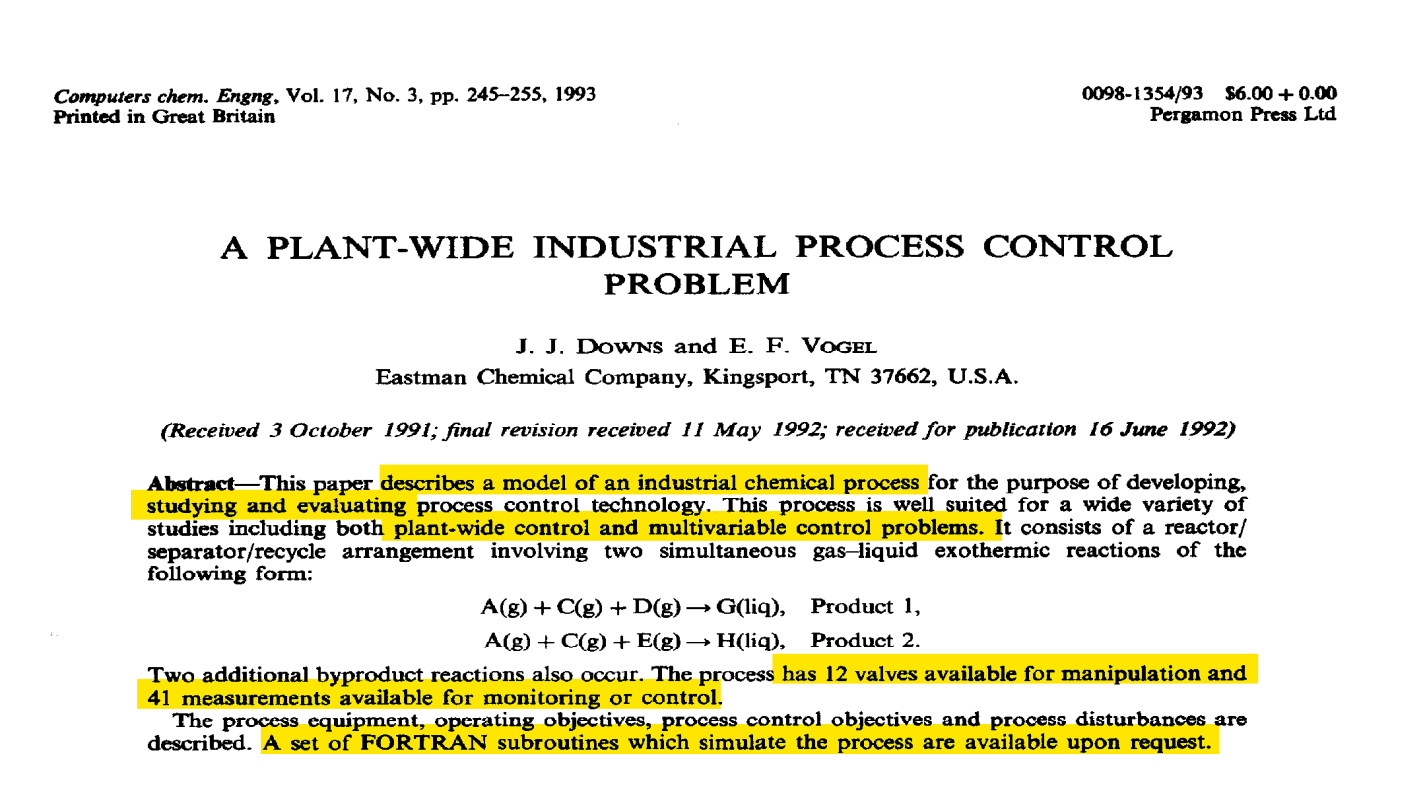
\includegraphics[width=0.74\textwidth]{art_1_capa}
\fonte{Downs e Vogel (1993), \textit{Computers \& Chemical Engineering}. Destaques do autor.}
\end{frame}

% ---------------------------------------------------------------------------
\begin{frame}{A planta: Processo Tennessee Eastman}
\marcador{A planta: Processo Tennessee Eastman}
\apendices{\irpara{ap-modos}{Modos}\irpara{ap-disturbios}{Distúrbios}}
\begin{columns}[T]
\column{0.60\textwidth}
\vspace{4pt}
\includegraphics[width=\linewidth]{tep-fluxograma}
\fonte{Downs e Vogel (1993).}
\column{0.37\textwidth}
\vspace{6pt}
\begin{itemize}\setlength{\itemsep}{6pt}
  \item Downs e Vogel (1993): um problema aberto de controle da planta inteira
  \item 5 unidades, reações não lineares e reciclo
  \item 20 distúrbios pré-definidos
  \item Modo~1: G/H 50/50
\end{itemize}
\end{columns}
\end{frame}

% ---------------------------------------------------------------------------
\begin{frame}{Camadas de controle}
\marcador{Camadas de controle}
\apendices{\irpara{ap-otimo}{Ponto ótimo}}
\vspace{2pt}
\begin{tikzpicture}[font=\scriptsize,
    comp/.style={draw=cinza, fill=white, rounded corners=1pt, align=center, inner sep=3pt, text=cinza, minimum height=0.6cm},
    escuro/.style={comp, fill=cinza, draw=cinza, text=white},
    faixa/.style={line width=3pt, gray!22},
    rot/.style={anchor=west, align=left, text=cinza},
    seta/.style={-{Latex[length=1.6mm]}, thick, cinza},
    duplaseta/.style={{Latex[length=1.6mm]}-{Latex[length=1.6mm]}, thick, cinza}]
  % faixas
  \draw[faixa] (0,-1.0) -- (13.2,-1.0);
  \draw[faixa] (0,-3.2) -- (13.2,-3.2);
  \draw[faixa] (0,-4.4) -- (13.2,-4.4);
  \node[rot] at (0,-0.5)  {\textbf{Otimização}\\(horas)};
  \node[rot] at (0,-2.1)  {\textbf{Controle}\\\textbf{supervisório}\\(minutos)};
  \node[rot] at (0,-3.8)  {\textbf{Controle}\\\textbf{regulatório}\\(segundos)};
  \node[rot] at (0,-4.95) {\textbf{Planta}};

  % otimização
  \node[comp, dashed] (opt) at (3.9,-0.5) {\texttt{tep-optimizer}};
  \node[anchor=west, text=cinza!80, font=\tiny] at (opt.east) {\ projeto paralelo, fora do escopo};

  % supervisório
  \node[comp] (his) at (3.9,-2.15) {\textit{historian}\\(Python)};
  \draw[dashed, gray!70, rounded corners=2pt] (5.3,-1.35) rectangle (10.4,-2.85);
  \node[anchor=north west, text=cinza!80, font=\tiny] at (5.3,-1.35) {cluster Kubernetes (Kind)};
  \node[escuro] (sup) at (6.75,-2.25) {\texttt{plant-supervisor}\\(Go)};
  \node[comp, font=\tiny] (rec) at (9.2,-2.25) {\texttt{Plant}\\\texttt{OperatingPolicy}\\\texttt{CostFunction}};
  \draw[seta] (sup) -- node[above, font=\tiny] {lê} (rec);
  \draw[seta] (sup.west) -- node[above, font=\tiny] {HTTP} (his.east);
  \node[comp] (ihm) at (12.35,-2.15) {IHM\\(Python)};
  \draw[seta] (10.4,-2.15) -- node[above, font=\tiny, pos=0.62] {veredito} (ihm.west);
  \draw[dashed, vermelho, thick, rounded corners=3pt] (3.05,-1.22) rectangle (10.55,-2.98);
  \node[anchor=south east, text=vermelho, font=\tiny\bfseries, fill=white, inner sep=1pt] at (10.55,-1.22) {foco deste trabalho};

  % regulatório e planta: o tep-plant
  \draw[draw=cinza, fill=cinzaClaro, rounded corners=2pt] (3.05,-3.4) rectangle (12.9,-5.45);
  \node[anchor=north east, text=cinza, font=\tiny] at (12.9,-3.4) {\texttt{tep-plant} (Rust)};
  \node[comp, minimum width=4.2cm] (mal) at (7.9,-3.85) {malhas P e PI: pressão e níveis};
  \node[comp, minimum width=4.2cm] (pro) at (7.9,-4.95) {processo do TEP, sensores e atuadores};
  \draw[duplaseta] (mal) -- (pro);

  % OPC UA
  \draw[duplaseta] (his.south) -- node[right, font=\tiny, pos=0.75] {OPC UA} (his.south |- 0,-3.4);
  \draw[duplaseta] (ihm.south) -- node[left, font=\tiny, pos=0.75] {OPC UA} (ihm.south |- 0,-3.4);
\end{tikzpicture}
\fonte{Camadas de Larsson e Skogestad (2000) e Skogestad (2004). Formato adaptado de Koziolek, Burger e Peedikayil (2024).}
\end{frame}

% ---------------------------------------------------------------------------
\begin{frame}{Cinco problemas e a política de operação}
\marcador{Cinco problemas e a política de operação}
\apendices{\irpara{ap-otimo}{Ponto ótimo}\irpara{ap-custo}{Função de custo}}
\begin{columns}[T]
\column{0.50\textwidth}
\centering
\vspace{10pt}
\begin{tikzpicture}[font=\scriptsize, scale=0.47, every node/.style={transform shape},
    fluxo/.style={-{Latex[length=2mm]}, thick, cinza}]
  \draw[cinza, thick] (0,0) circle (2.5); \draw[cinza, thick] (4.0,0) circle (2.5); \draw[cinza, thick] (8.0,0) circle (2.5);
  \draw[cinza, fill=cinzaClaro] (0,-1.2) circle (1.15);
  \node[align=center, font=\large, text=cinza] at (0,0.7)   {\textbf{P1}\\Otimização};
  \node[align=center, font=\normalsize, text=cinza] at (0,-1.2)  {\textbf{P2}\\Estabilidade};
  \node[align=center, font=\large, text=cinza] at (4.0,0.7) {\textbf{P3}\\\textit{Self-optimizing}};
  \node[align=center, font=\large, text=cinza] at (8.0,0.7) {\textbf{P4}\\Controle};
  \draw[fluxo] (2.0,-0.4) -- (2.0,-3.2) node[below, font=\normalsize, text=cinza] {ponto ótimo};
  \draw[fluxo] (6.0,-0.4) -- (6.0,-3.2) node[below, font=\normalsize, text=cinza] {setpoints};
  \draw[dashed, vermelho, very thick, rounded corners=4pt] (-3.1,-4.2) rectangle (11.1,3.4);
  \node[anchor=south, font=\Large, text=vermelho] at (4.0,3.4) {\textbf{P5 Supervisão}};
\end{tikzpicture}
\column{0.47\textwidth}
\vspace{4pt}
\destaque{\textbf{Política de operação}: o que P1 a P4 dizem sobre como a planta deveria operar.\\[2pt]
\footnotesize O que produzir, por onde não passar, quanto deve custar e quais malhas devem funcionar.}\par
\vspace{-6pt}
\begin{itemize}\setlength{\itemsep}{4pt}
  \item P1 a P4: já estão na literatura
  \item Falta o \textbf{P5}: acompanhar a política com a planta em operação
\end{itemize}
\end{columns}
\end{frame}

% ---------------------------------------------------------------------------
\begin{frame}{De onde vem o Kubernetes}
\marcador{De onde vem o Kubernetes}
\centering
\vspace{2pt}
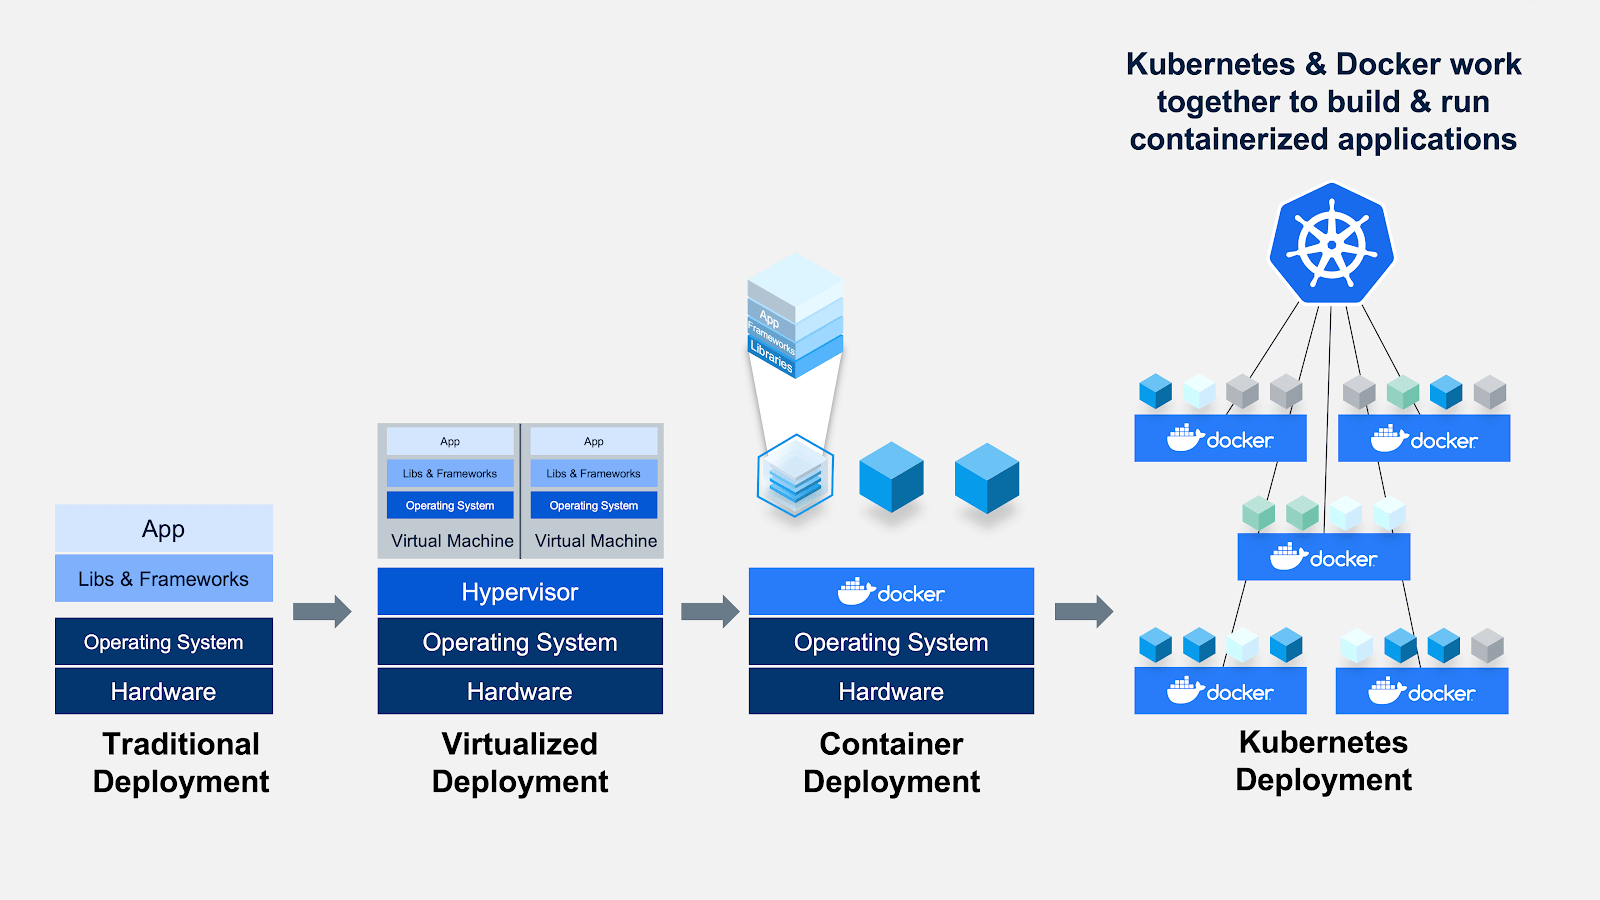
\includegraphics[width=0.68\textwidth]{tradicional_k8s}\par
\vspace{4pt}
\begin{minipage}{0.68\textwidth}
\raggedright\small Com muitos \textit{containers} em várias máquinas, alguém precisa decidir onde cada um roda e recriá-lo quando ele cai. Esse é o papel do Kubernetes.
\end{minipage}
\end{frame}

% ---------------------------------------------------------------------------
\begin{frame}{Por que o Kubernetes}
\marcador{Por que o Kubernetes}
\begin{columns}[T]
\column{0.57\textwidth}
\centering
\vspace{2pt}
\begin{tikzpicture}[font=\scriptsize,
    caixa/.style={draw=cinza, fill=white, align=center, text=cinza, inner sep=3pt, minimum height=0.55cm},
    escuro/.style={caixa, fill=cinza, text=white},
    seta/.style={-{Latex[length=1.6mm]}, thick, cinza},
    duplaseta/.style={{Latex[length=1.6mm]}-{Latex[length=1.6mm]}, thick, cinza},
    plano/.style={fill=cinzaClaro, draw=gray!50}]
  % usuário
  \node[caixa, fill=cinzaClaro] (usr) at (4.9,0) {\textbf{Usuário}\\\texttt{\$ kubectl apply -f politica.yaml}};

  % control plane
  \draw[plano] (0,-0.6) rectangle (7.3,-3.2);
  \node[anchor=north west, text=cinza] at (0.1,-0.62) {\textbf{\textit{Control plane}}};
  \node[caixa, minimum width=2.6cm] (api)  at (5.15,-1.25) {servidor de API};
  \node[caixa, minimum width=2.6cm] (etcd) at (5.15,-1.95) {etcd: \textit{Spec} e \textit{Status}};
  \node[caixa, minimum width=2.6cm] (nat)  at (5.15,-2.65) {controladores nativos};
  \node[caixa, rounded corners=3pt] (crd) at (1.55,-1.55) {recurso próprio\\(CRD)};
  \node[escuro] (op) at (1.75,-2.55) {operador\\(controlador próprio)};
  \draw[seta] (usr.south -| api.north) -- (api.north);
  \draw[seta] (api.west) -- (crd.east);
  \draw[duplaseta] (op.east) -- (api.south west);
  \node[font=\tiny, text=cinza] at (3.1,-2.0) {compara};
  \draw[thick, cinza] (api) -- (etcd);
  \draw[duplaseta, rounded corners=2pt] (api.east) -- ++(0.45,0) |- (nat.east);

  % nós
  \draw[plano] (0,-3.45) rectangle (7.3,-4.65);
  \foreach \x in {1.4,3.65,5.9}
    \node[caixa, minimum width=1.4cm] at (\x,-3.95) {\textit{pods}};
  \node[anchor=south, text=cinza] at (3.65,-4.65) {\textbf{Nós}};
  \draw[seta] (nat.south) -- node[right, font=\tiny] {cria e recria} (nat.south |- 0,-3.45);
\end{tikzpicture}
\fonte{Formato adaptado de Koziolek, Burger e Peedikayil (2024).}
\column{0.40\textwidth}
\vspace{2pt}
\begin{itemize}\setlength{\itemsep}{5pt}
  \item \textit{Spec} (desejado) e \textit{Status} (observado); controladores comparam os dois
  \item CRD com controlador próprio: o padrão \textit{Operator}
  \item Aqui: desejado = política; observado = planta
  \item Não é tempo real, e não precisa ser
\end{itemize}
\end{columns}
\end{frame}

% ---------------------------------------------------------------------------
\begin{frame}{Objetivo}
\marcador{Objetivo}
\vspace{2pt}
\begin{tikzpicture}\node[fill=cinzaClaro,rounded corners=3pt,inner sep=7pt,text width=\linewidth-14pt,align=flush left]{%
{\color{verdeEsc}\textbf{Objetivo geral}}\hfill{\scriptsize\color{cinza}Ênfase: Integração de Sistemas de Controle}\\[2pt]
\small Mostrar que uma camada supervisória construída sobre o Kubernetes consegue acompanhar uma planta a partir de uma \textbf{política declarada pelo usuário}, sem que o supervisor conheça a planta.};\end{tikzpicture}
\par\vspace{2pt}
\begin{columns}[T]
\column{0.58\textwidth}
{\color{verdeEsc}\small\textbf{Objetivos específicos}}
\begin{enumerate}\setlength{\itemsep}{1pt}\small
  \item TEP contínuo, em OPC~UA, fiel ao original
  \item \textit{Historian} com estatísticas dos sinais
  \item Política do Modo~1 declarada no Kubernetes
  \item Veredito em operação normal e sob IDV(6)
  \item IHM com a planta e o veredito
\end{enumerate}
\column{0.40\textwidth}
\begin{tikzpicture}\node[fill=cinzaClaro,rounded corners=3pt,inner sep=6pt,text width=\linewidth-12pt,align=flush left]{%
{\color{cinza}\textbf{Fora do escopo}}\par\vspace{3pt}
{\footnotesize\setlength{\parskip}{2pt}
$\cdot$ escolher variáveis controladas\par
$\cdot$ sintonizar controladores\par
$\cdot$ resolver P1 a P4\par
$\cdot$ agir sobre a planta\par}};\end{tikzpicture}
\end{columns}
\end{frame}

% ===========================================================================
\divisor{O que foi construído}{Planta, \textit{historian}, supervisor e IHM}

% ---------------------------------------------------------------------------
\begin{frame}{O laboratório}
\marcador{O laboratório}
\apendices{\irpara{ap-containers}{Containers}}
\centering
\vspace{2pt}
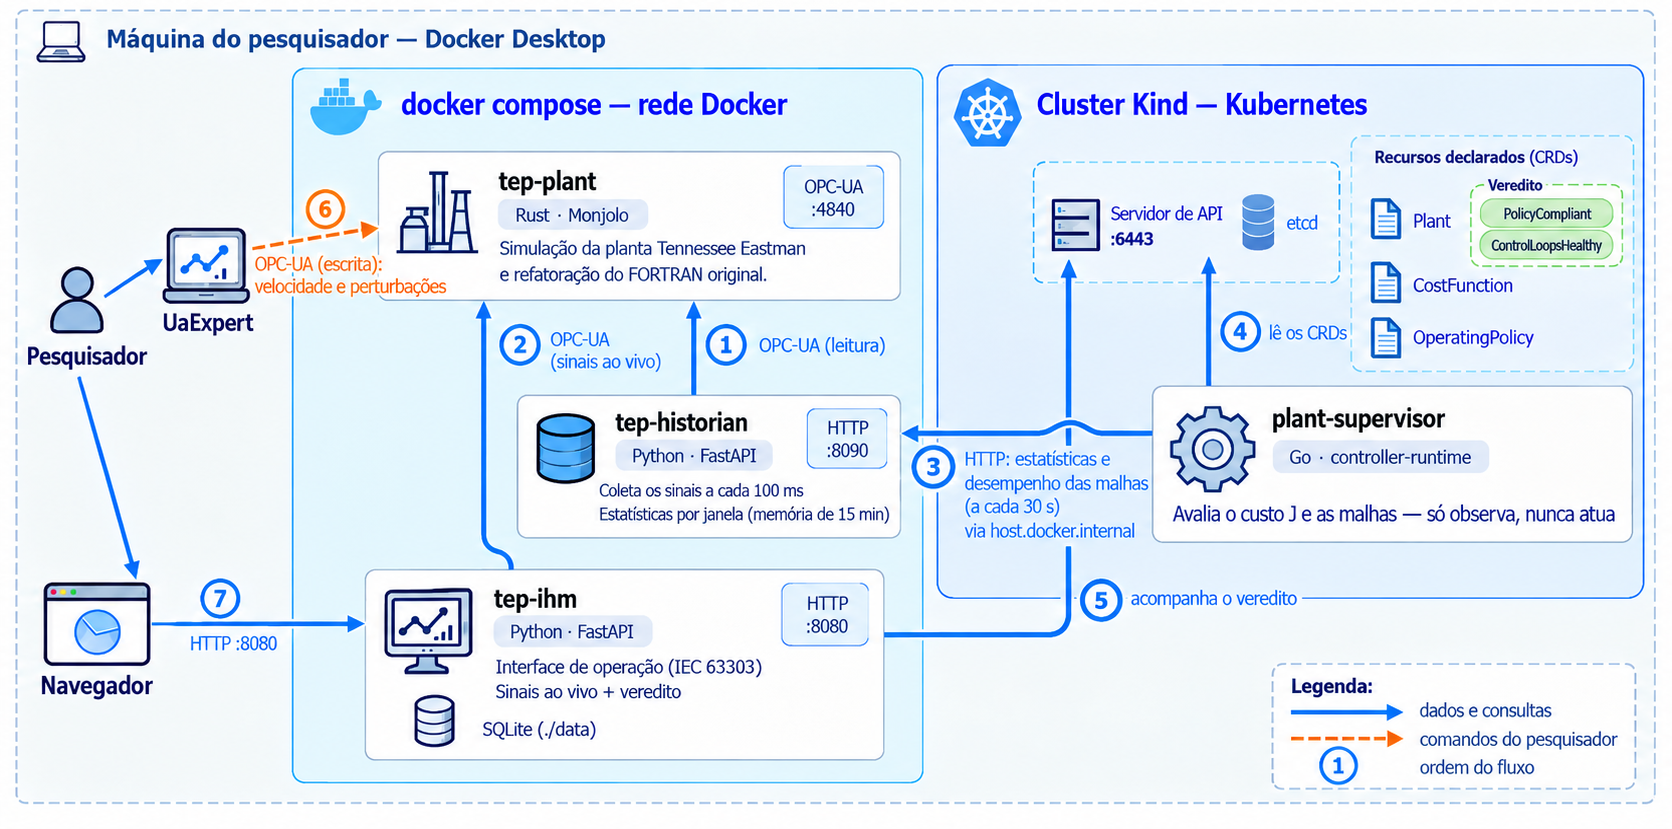
\includegraphics[width=0.84\textwidth]{arquitetura}
\fonte{A planta fica fora do Kubernetes; o \textit{cluster} só observa.}
\end{frame}

% ---------------------------------------------------------------------------
\begin{frame}{A planta simulada}
\marcador{A planta simulada}
\apendices{\irpara{ap-fortran}{Código FORTRAN}\irpara{ap-tep-plant}{tep-plant}}
\begin{columns}[T]
\column{0.44\textwidth}
\vspace{4pt}
\begin{itemize}\setlength{\itemsep}{6pt}
  \item FORTRAN de Downs e Vogel reescrito em \textbf{Rust}, sobre um \textit{framework} próprio (monjolo)
  \item Roda de forma \textbf{contínua}
  \item Publica os sinais por \textbf{OPC~UA} (IEC~62541)
  \item Velocidade e distúrbios comandados pelo OPC~UA, até \textasciitilde56$\times$ o tempo real
\end{itemize}
\column{0.53\textwidth}
\vspace{4pt}
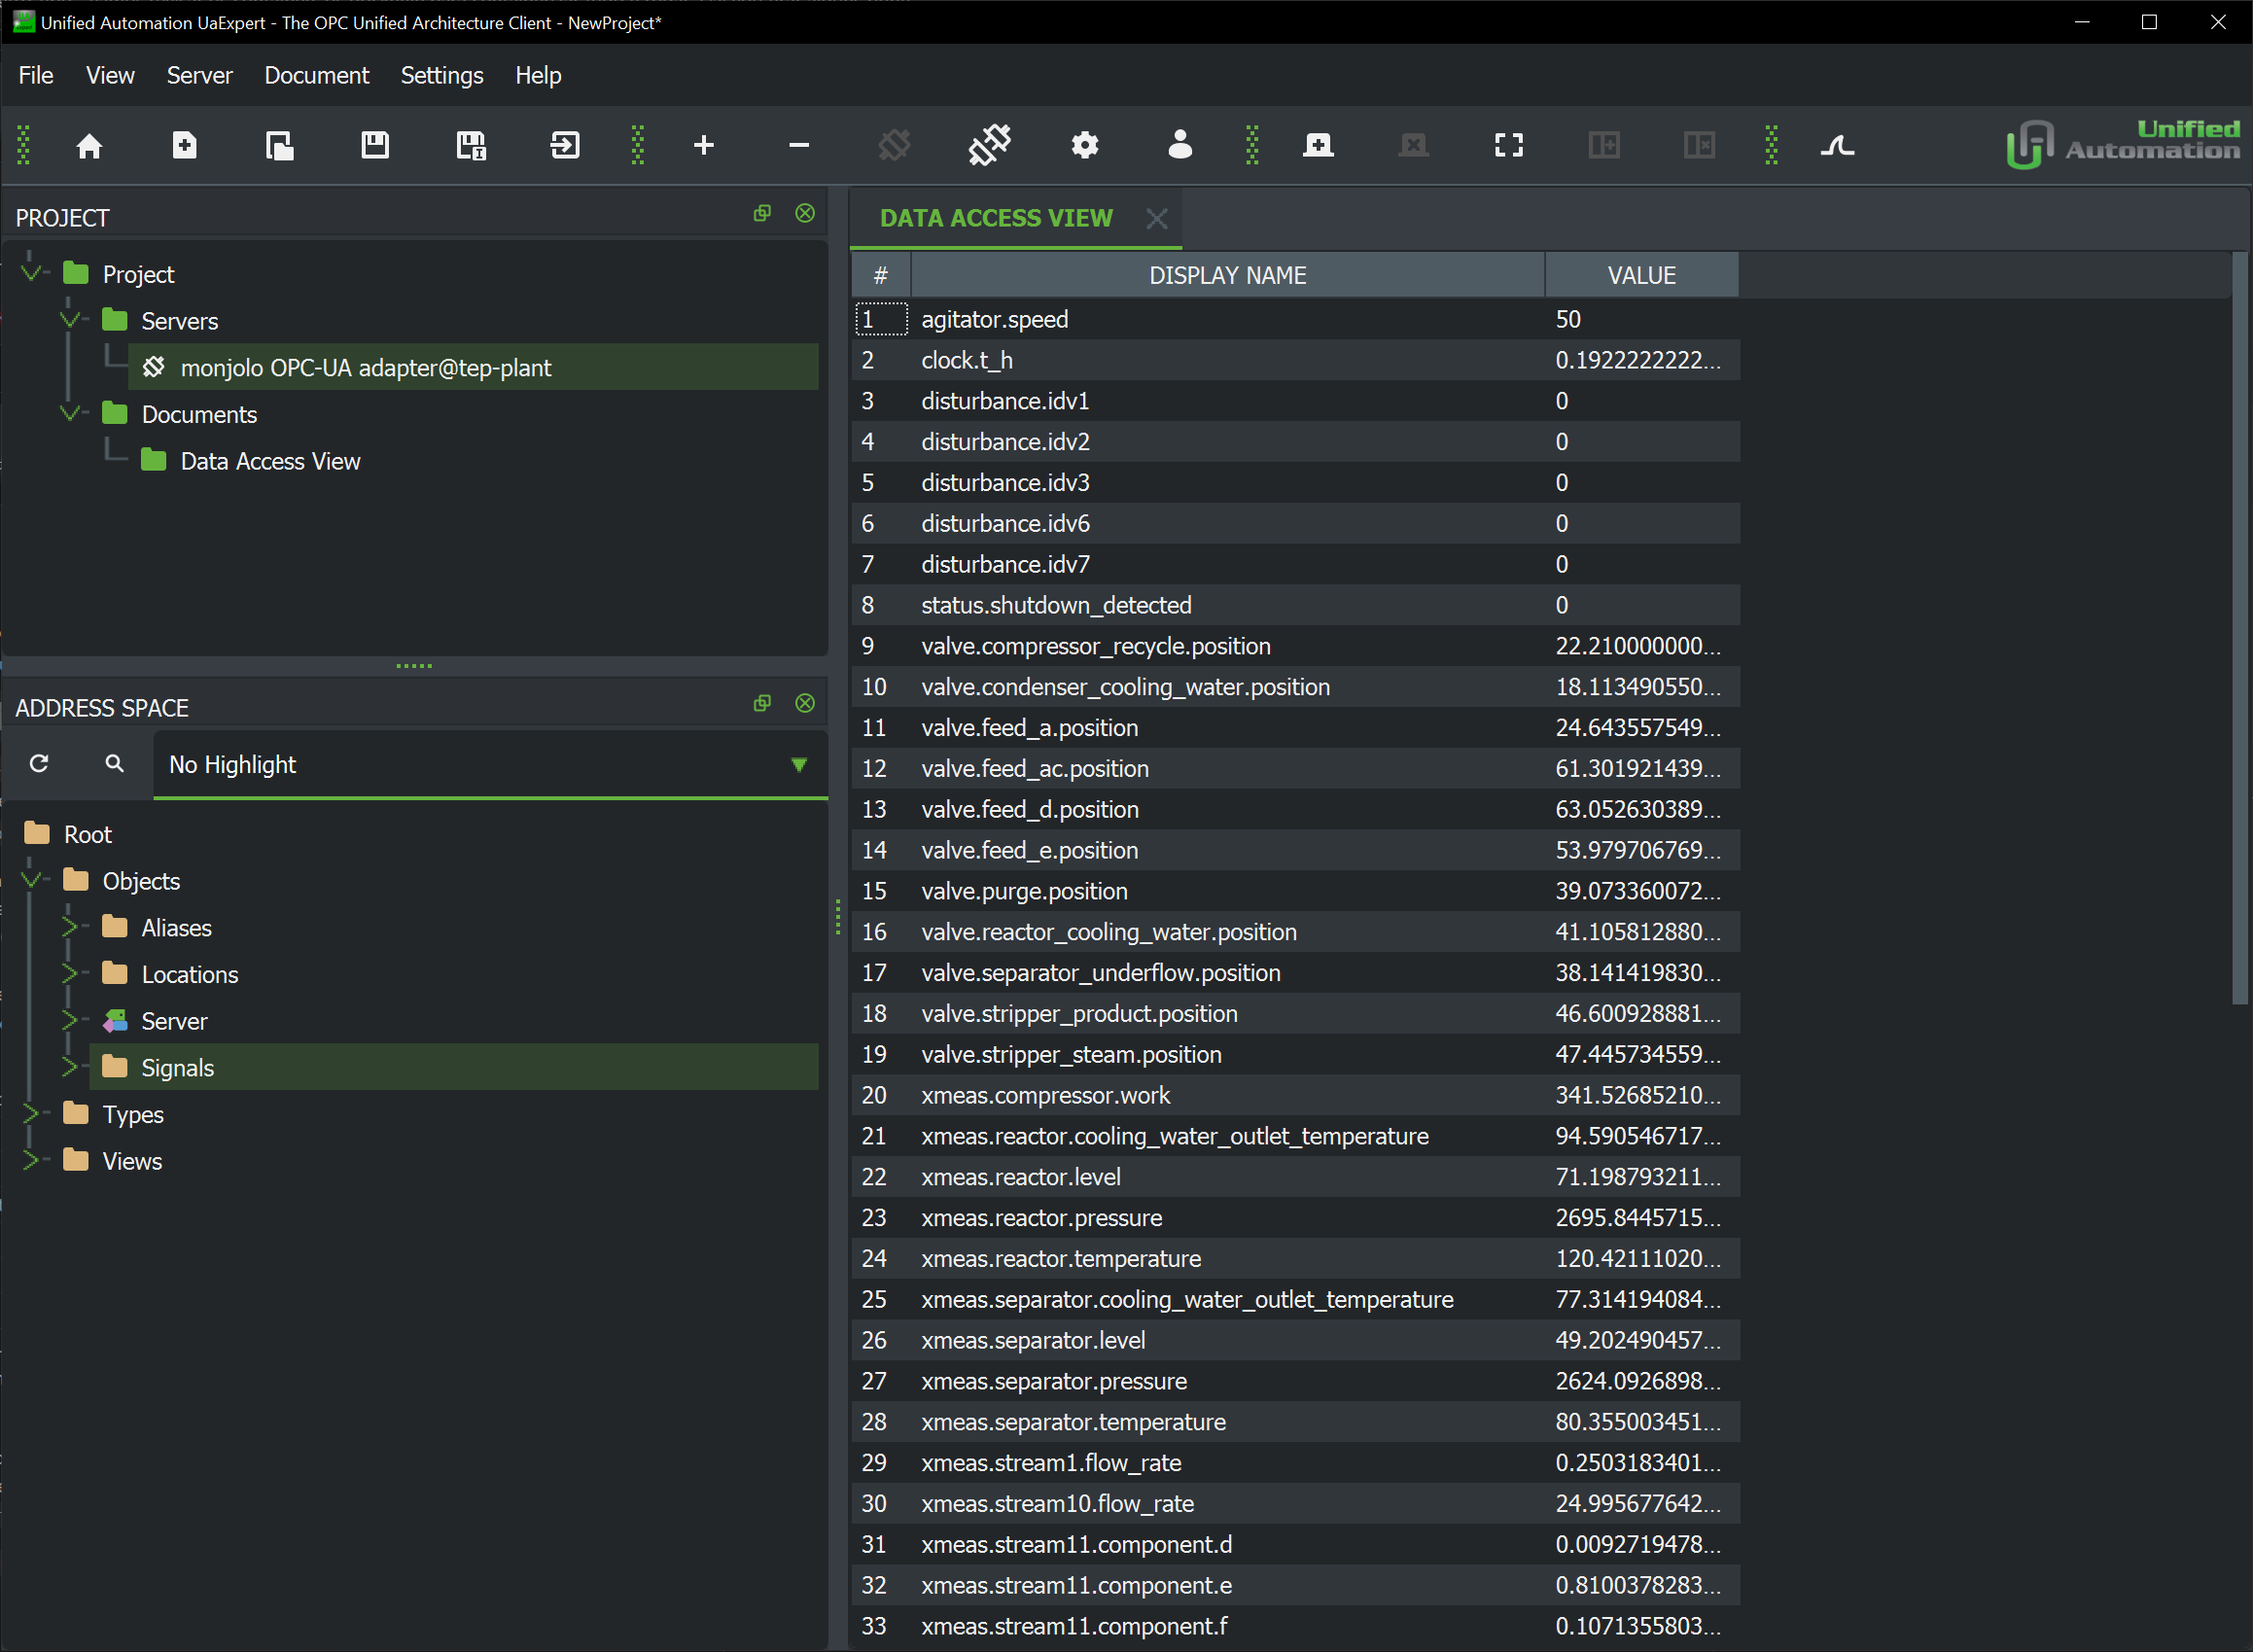
\includegraphics[width=0.9\linewidth]{uaexpert}
\fonte{A planta vista pelo UaExpert, um cliente OPC~UA comercial.}
\end{columns}
\end{frame}

% ---------------------------------------------------------------------------
\begin{frame}{\textit{Historian}}
\marcador{Historian}
\apendices{\irpara{ap-preditividade}{Erro previsível}}
\begin{columns}[T]
\column{0.50\textwidth}
\vspace{6pt}
\begin{itemize}\setlength{\itemsep}{6pt}
  \item Em Python; coleta todos os sinais a cada 100~ms, por OPC~UA
  \item Guarda 15~min em memória
  \item Responde por HTTP:
  \begin{itemize}
    \item \texttt{/aggregate}: média e desvio padrão de cada sinal numa janela
    \item \texttt{/loop-performance}: índice de cada malha
  \end{itemize}
\end{itemize}
\column{0.47\textwidth}
\vspace{6pt}
\destaque{\textbf{Índice das malhas}\\{\footnotesize Bradu \textit{et al.} (2018), CERN}\\[4pt]
\footnotesize Ajusta um modelo autorregressivo ao erro da malha. Se o erro é \textbf{previsível}, há algo a melhorar na malha.\\[3pt]
Só é julgada a malha cuja válvula se mexe: malhas paradas, saturadas ou em manual ficam de fora.}
\end{columns}
\end{frame}

% ---------------------------------------------------------------------------
\begin{frame}[fragile]{Supervisor: três recursos declarados}
\marcador{Recursos: Plant}
\begin{columns}[T]
\column{0.42\textwidth}
\centering
\vspace{6pt}
\fluxoRecursos{1}
\column{0.56\textwidth}
\vspace{2pt}
{\small\textcolor{recPlant}{\textbf{\texttt{plant.yaml}}}}\hfill{\tiny\color{cinza!80}completo, sem os comentários}
\lstset{backgroundcolor=\color{recPlant!8}, escapeinside={(*@}{@*)}}
\begin{lstlisting}
apiVersion: supervision.greenlabs.io/v1alpha1
kind: Plant
metadata:
  (*@\grifo{recPlant}{name: tep}@*)
spec:
  historianURL: "http://host.docker.internal:8090"
  (*@\grifo{recPolicy}{policyRef: tep-mode1}@*)
  evaluationIntervalSeconds: 30
\end{lstlisting}
\fonte{Trocar de política é trocar o \texttt{policyRef}.}
\end{columns}
\end{frame}

% ---------------------------------------------------------------------------
\begin{frame}[fragile]{Supervisor: três recursos declarados}
\marcador{Recursos: OperatingPolicy}
\begin{columns}[T]
\column{0.42\textwidth}
\centering
\vspace{6pt}
\fluxoRecursos{2}
\column{0.56\textwidth}
\vspace{2pt}
{\small\textcolor{recPolicy}{\textbf{\texttt{policy-mode1.yaml}}}}\hfill{\tiny\color{cinza!80}trechos}
\lstset{backgroundcolor=\color{recPolicy!8}, escapeinside={(*@}{@*)}}
\begin{lstlisting}
kind: OperatingPolicy
metadata:
  (*@\grifo{recPolicy}{name: tep-mode1}@*)
spec:
  (*@\grifo{recCost}{costFunctionRef: tep-downs-vogel}@*)
  maxCost: 170.6        # $/h, caso base
  persistenceEvaluations: 3
  targets:
    - signal: xmeas.stream11.flow_rate
      value: 22.949     # m3/h, +-5 %
  # ... 5 limites (pressao, temperatura, niveis)
  controlLoops:
    - name: separator_level
      setpoint: 50
      minPredictability: 0.12
\end{lstlisting}
\end{columns}
\end{frame}

% ---------------------------------------------------------------------------
\begin{frame}[fragile]{Supervisor: três recursos declarados}
\marcador{Recursos: CostFunction}
\begin{columns}[T]
\column{0.42\textwidth}
\centering
\vspace{6pt}
\fluxoRecursos{3}
\column{0.56\textwidth}
\vspace{2pt}
{\small\textcolor{recCost}{\textbf{\texttt{cost-function-downs-vogel.yaml}}}}\hfill{\tiny\color{cinza!80}trechos}
\lstset{backgroundcolor=\color{recCost!8}, escapeinside={(*@}{@*)}}
\begin{lstlisting}
kind: CostFunction
metadata:
  (*@\grifo{recCost}{name: tep-downs-vogel}@*)
spec:
  unit: "$/h"
  reference: 170.6
  terms:
    - name: purge.a
      coefficient: 0.9880674   # 2.206 x 44.79 / 100
      signals: [xmeas.stream9.flow_rate,
                xmeas.stream9.component.a]
    # ... mais 11 termos: purga, produto,
    #     compressor e vapor
\end{lstlisting}
\end{columns}
\apendices{\irpara{ap-custo}{Função de custo}}
\end{frame}

% ---------------------------------------------------------------------------
\begin{frame}[fragile]{O veredito}
\marcador{O veredito}
\begin{columns}[T]
\column{0.56\textwidth}
A cada 30~s, o supervisor:
\begin{enumerate}\setlength{\itemsep}{1pt}
  \item pede ao \textit{historian} as médias da janela
  \item calcula $J$ e confere orçamento, metas e limites
  \item julga cada malha: índice e \textit{offset}
  \item grava tudo no \textit{status} da \texttt{Plant}
\end{enumerate}
\vspace{3pt}
{\small Três avaliações ruins seguidas $\Rightarrow$ \textcolor{vermelhoIF}{\textbf{\texttt{NonCompliant}}}}
\vspace{4pt}
\begin{lstlisting}
$ kubectl get plants
NAME  POLICY     COST    PHASE      LOOPS
tep   tep-mode1  166.39  Compliant  True
\end{lstlisting}
\vspace{2pt}
{\small O supervisor \textbf{nunca escreve na planta}.}
\column{0.40\textwidth}
\centering
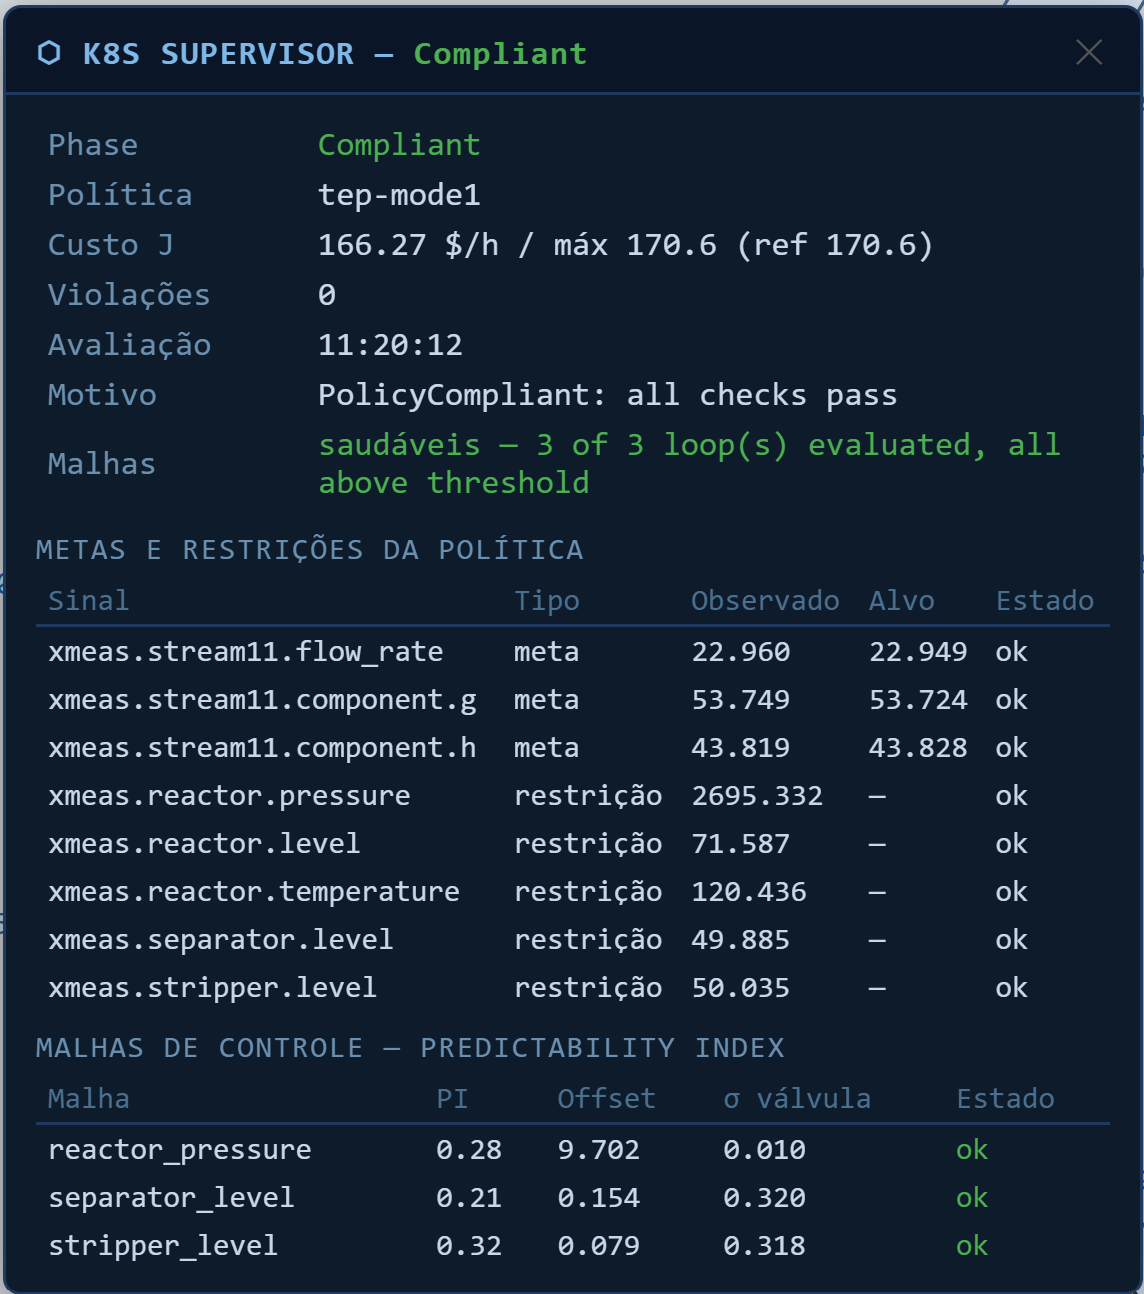
\includegraphics[height=0.64\textheight]{ihm-painel-k8s}
\fonte{O mesmo \textit{status} no painel da IHM.}
\end{columns}
\end{frame}

% ---------------------------------------------------------------------------
\begin{frame}{IHM}
\marcador{IHM}
\centering
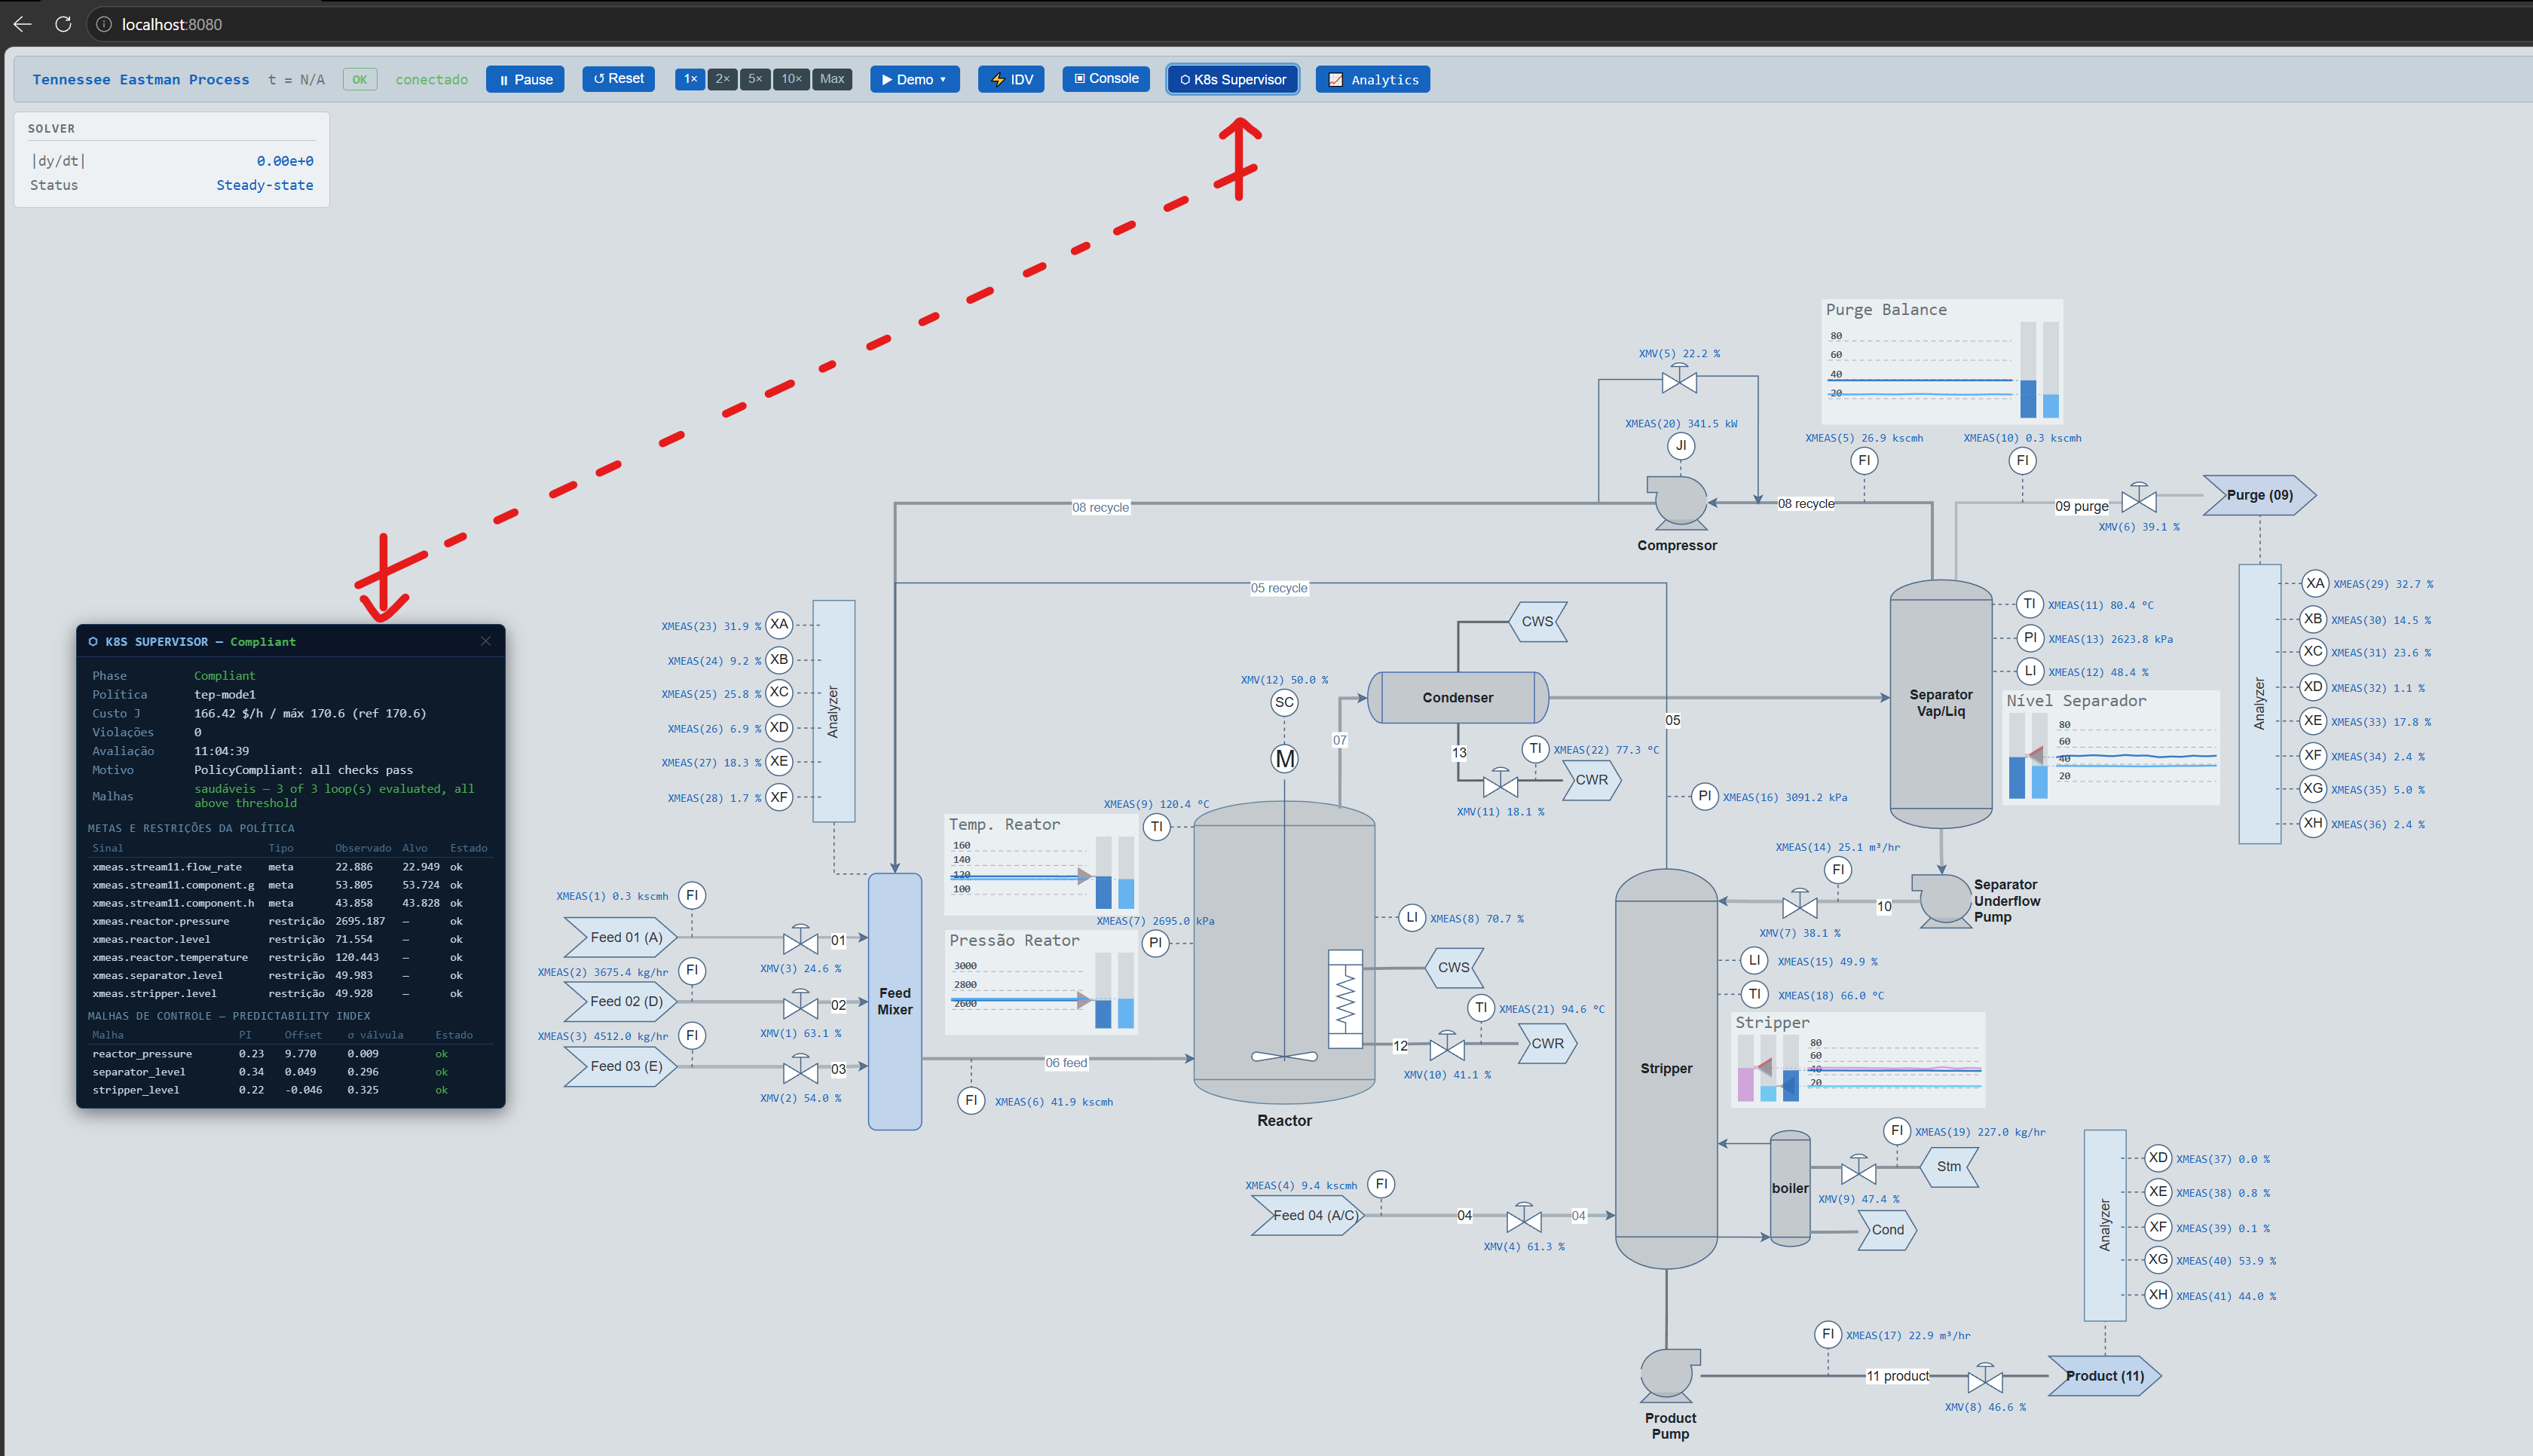
\includegraphics[height=0.66\textheight]{ihm-com-k8s}
\fonte{Aplicação web: sinais ao vivo por OPC~UA e o veredito lido do Kubernetes.}
\end{frame}

% ===========================================================================
\divisor{Resultados}{A planta simulada e o veredito do supervisor}

% ---------------------------------------------------------------------------
\begin{frame}{A planta simulada e o modelo original}
\marcador{A planta simulada e o modelo original}
\apendices{\irpara{ap-otimo}{Ponto ótimo}\irpara{ap-parcelas}{Custo por parcela}}
\vspace{6pt}
\centering
\begin{tikzpicture}[
    card/.style={fill=cinzaClaro, rounded corners=4pt, minimum width=5.6cm, minimum height=3.0cm, text width=5.2cm, align=center}]
  \node[card] at (0,0) {%
    {\footnotesize\color{verdeIF}\textbf{CASO BASE}\\Downs e Vogel (1993)\par}\vspace{4pt}
    {\fontsize{24}{26}\selectfont\bfseries\color{verdeEsc} 170,63\par}
    {\footnotesize \$/h na planta\par}\vspace{4pt}
    {\small contra \textbf{170,61}~\$/h publicados\par}};
  \node[card] at (6.2,0) {%
    {\footnotesize\color{verdeIF}\textbf{ÓTIMO DO MODO~1}\\Ricker (1995)\par}\vspace{4pt}
    {\fontsize{24}{26}\selectfont\bfseries\color{verdeEsc} 114,32\par}
    {\footnotesize \$/h encontrado\par}\vspace{4pt}
    {\small contra \textbf{114,31}~\$/h publicados\par}};
\end{tikzpicture}\par
\vspace{12pt}
\begin{minipage}{0.86\textwidth}
\begin{itemize}\setlength{\itemsep}{2pt}
  \item Caso base: derivadas dos 50 estados perto de zero; as 41 medições batem com o artigo
  \item Ótimo: as 12 válvulas a menos de 0,001 ponto percentual das publicadas
\end{itemize}
\end{minipage}
\end{frame}

% ---------------------------------------------------------------------------
\begin{frame}{Os experimentos ao longo de 2026}
\marcador{Os experimentos ao longo de 2026}
\centering
\vspace{4pt}
\begin{tikzpicture}[font=\scriptsize,
    fase/.style={draw=gray!45, fill=white, rounded corners=3pt, text width=2.75cm, minimum height=3.0cm,
                 align=center, inner sep=4pt, text=gray!60, anchor=north},
    usada/.style={fase, draw=verdeIF, fill=cinzaClaro, thick, text=cinza},
    principal/.style={fase, draw=verdeEsc, fill=verdeIF!12, very thick, text=cinza},
    data/.style={font=\tiny, text=cinza}]
  % linha do tempo
  \draw[-{Latex[length=2mm]}, thick, gray!50] (-0.2,0) -- (12.9,0);
  \foreach \x/\d in {1.55/mar, 4.75/abr a jun, 7.95/set, 11.15/out}
    { \fill[gray!50] (\x,0) circle (2pt); \node[data, above] at (\x,0.05) {\d}; }

  \node[usada] (f1) at (1.55,-0.3) {%
    {\Large\bfseries\color{verdeEsc} 1 a 11}\\[3pt]
    \textbf{Partida e linha de base}\\[2pt]
    {\tiny primeira versão em Rust, gravando CSV}\\[5pt]
    {\tiny\color{verdeIF}\textbf{Cap. 3}}};
  \node[fase] (f2) at (4.75,-0.3) {%
    {\Large\bfseries 12 a 17}\\[3pt]
    \textbf{Pilha integrada e distúrbios}\\[2pt]
    {\tiny versão anterior da planta; IDV(1) a IDV(4)}\\[5pt]
    {\tiny fora da monografia}};
  \node[fase] (f3) at (7.95,-0.3) {%
    {\Large\bfseries 18 a 24}\\[3pt]
    \textbf{Água de resfriamento}\\[2pt]
    {\tiny investigação do colapso térmico}\\[5pt]
    {\tiny fora da monografia}};
  \node[principal] (f4) at (11.15,-0.3) {%
    {\Large\bfseries\color{verdeEsc} 25 a 27}\\[3pt]
    \textbf{Supervisão pelo Kubernetes}\\[2pt]
    {\tiny IDV(6), seguimento do setpoint, malhas PI}\\[5pt]
    {\tiny\color{verdeIF}\textbf{Cap. 4: resultados}}};
\end{tikzpicture}
\par\vspace{8pt}
\begin{minipage}{0.84\textwidth}
\raggedright\small Um registro do projeto, em ordem cronológica: cada experimento tem observação, hipótese, intervenção, resultado e conclusão. Os 25, 26 e 27 são os únicos feitos com o supervisor no Kubernetes.
\end{minipage}
\end{frame}

% ---------------------------------------------------------------------------
\begin{frame}{Experimento 25: IDV(6), perda da alimentação de A}
\marcador{Experimento 25: IDV(6), perda da alimentação de A}
\apendices{\irpara{ap-disturbios}{Distúrbios}\irpara{ap-velocidade}{Velocidade e janelas}}
\begin{columns}[T]
\column{0.66\textwidth}
\vspace{4pt}
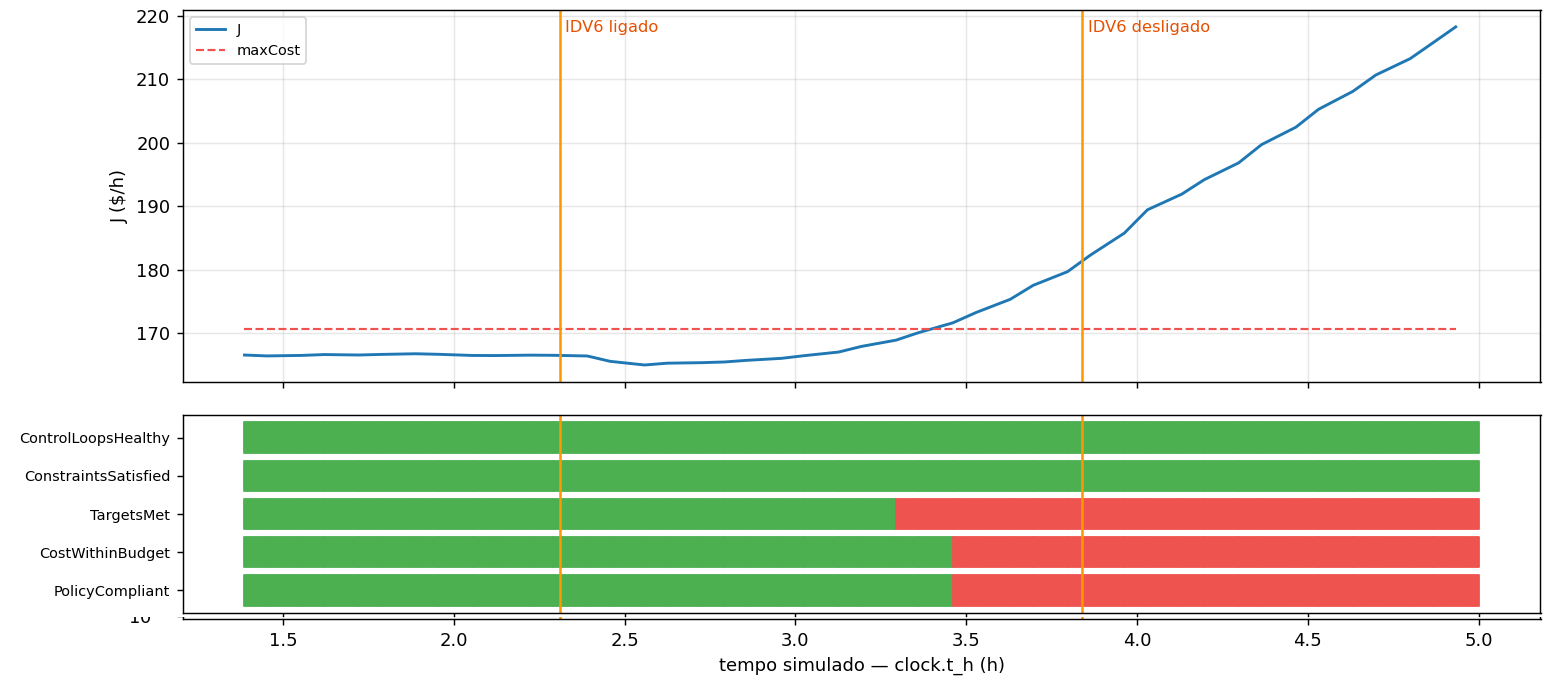
\includegraphics[width=\linewidth]{exp25-custo-conditions}
\fonte{Experimento 25: custo $J$ e \textit{conditions} do supervisor.}
\column{0.32\textwidth}
\vspace{2pt}
\begin{itemize}\setlength{\itemsep}{5pt}
  \item Operação normal: \texttt{Compliant} nas 41 avaliações
  \item \textbf{+0,98~h}: produto abaixo da meta
  \item \textbf{+1,15~h}: custo acima do orçamento, \textcolor{vermelhoIF}{\texttt{NonCompliant}}
  \item Na ordem física, com a política fixa
\end{itemize}
\end{columns}
\end{frame}

% ---------------------------------------------------------------------------
\begin{frame}{Experimento 26: critério de seguimento do \textit{setpoint}}
\marcador{Experimento 26: critério de seguimento do setpoint}
\begin{columns}[T]
\column{0.66\textwidth}
\vspace{4pt}
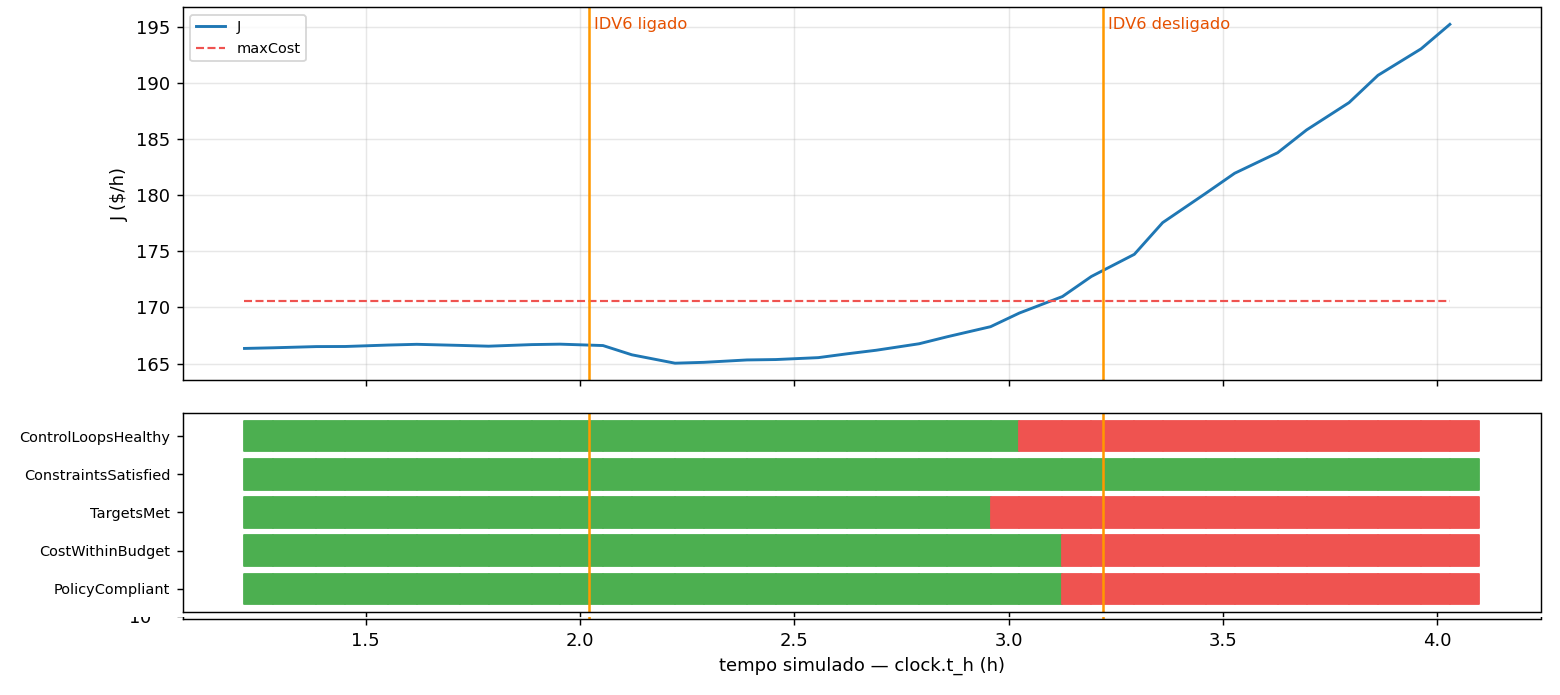
\includegraphics[width=\linewidth]{exp26-custo-conditions}
\fonte{Experimento 26: a mesma rodada, com o critério de seguimento do \textit{setpoint}.}
\column{0.32\textwidth}
\vspace{2pt}
\begin{itemize}\setlength{\itemsep}{5pt}
  \item Exp.~25: malhas ``saudáveis'' com a pressão 131~kPa acima do \textit{setpoint}
  \item Entrou o critério de \textbf{\textit{offset} máximo}
  \item Exp.~26: níveis, produto, malhas e custo, nessa ordem, de +0,84 a +1,11~h
\end{itemize}
\end{columns}
\end{frame}

% ---------------------------------------------------------------------------
\begin{frame}{A escala do índice das malhas}
\marcador{A escala do índice das malhas}
\begin{columns}[T]
\column{0.64\textwidth}
{\scriptsize\textbf{\color{vermelhoIF}Original:} como o supervisor gravou (escala do código, limite 0,12)}\par
\makebox[0.07\linewidth]{}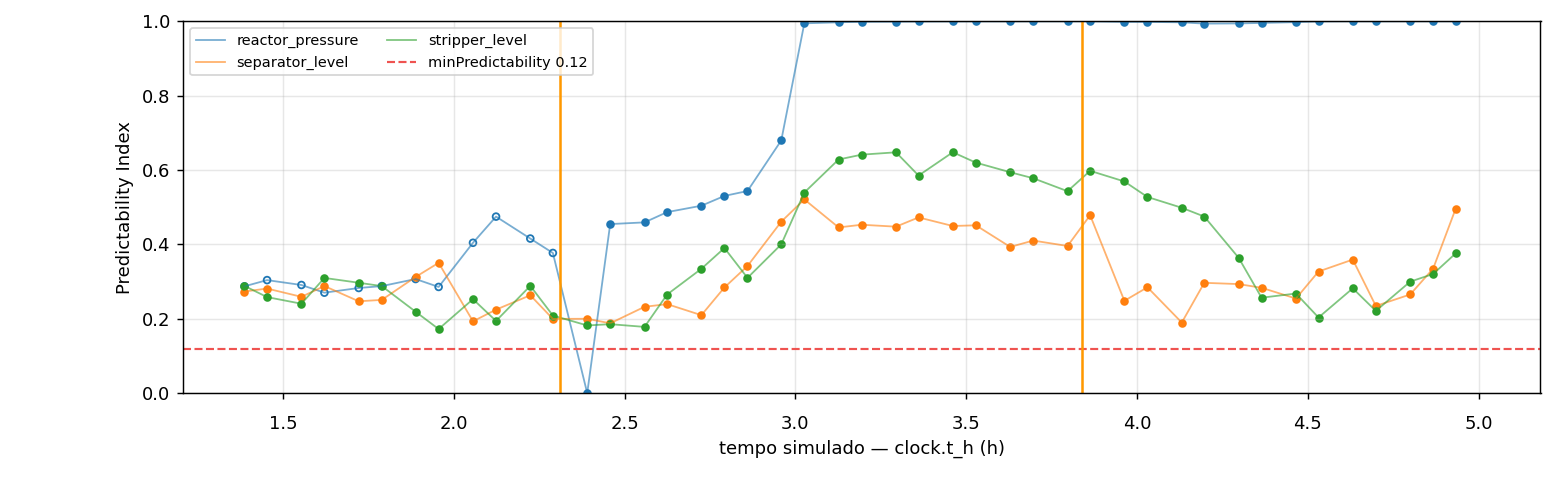
\includegraphics[width=0.90\linewidth]{exp25-indice-escala-codigo}\par
\vspace{3pt}
{\scriptsize\textbf{\color{verdeIF}Releitura:} os mesmos dados na escala do artigo (limite 0,5)}\par
\makebox[0.07\linewidth]{\raisebox{0.95cm}{%
  \tikz[scale=1.0]{%
    \draw[-{Latex[length=1.3mm]}, thick, cinza] (-0.28,0) -- (0.32,0);
    \node[font=\tiny, text=cinza, below] at (0.28,-0.02) {$x$};
    \draw[-{Latex[length=1.3mm]}, thick, verdeIF] (0.02,0.2) arc[start angle=90, end angle=-215, x radius=0.09, y radius=0.2];
    \node[font=\tiny, text=verdeIF, above] at (0.02,0.2) {180°};}}}%
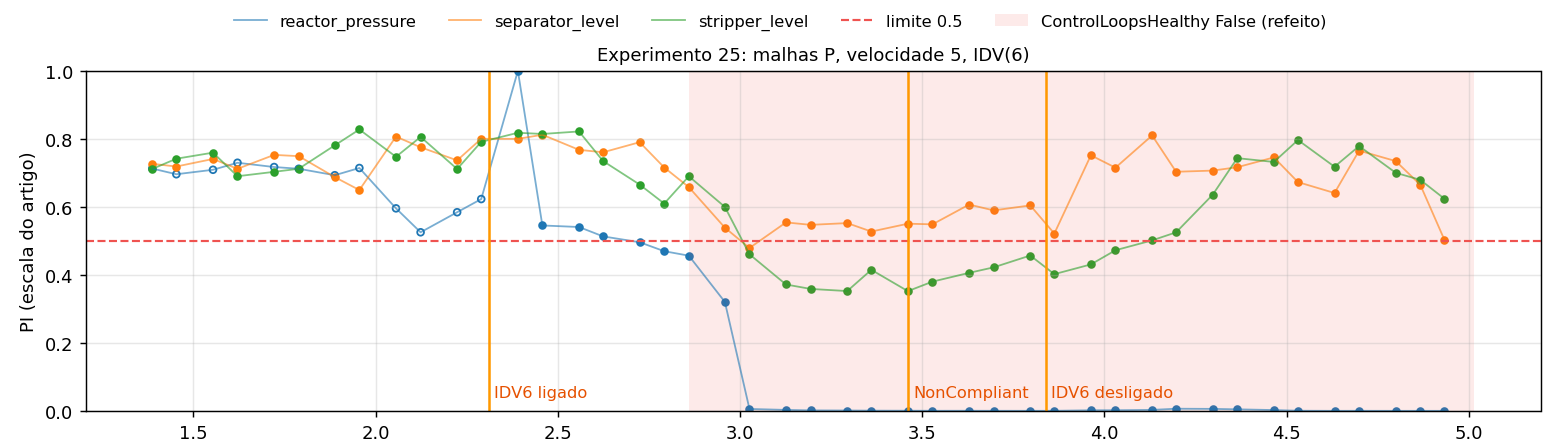
\includegraphics[width=0.90\linewidth]{releitura-exp25}
\column{0.33\textwidth}
\vspace{2pt}
\begin{itemize}\setlength{\itemsep}{5pt}
  \item O código gravava $1 - \text{índice}$
  \item Na escala certa: alarme em \textbf{+0,6~h}, antes do custo
  \item Mas também acusa transitórios inofensivos
  \item É \textbf{complemento} do \textit{offset} e dos limites, como no CERN
\end{itemize}
\end{columns}
\apendices{\irpara{ap-preditividade}{Erro previsível}}
\end{frame}

% ---------------------------------------------------------------------------
\begin{frame}{Experimento 27: malhas PI em operação normal}
\marcador{Experimento 27: malhas PI em operação normal}
\apendices{\irpara{ap-p-pi}{Malhas P e PI}}
\begin{columns}[T]
\column{0.54\textwidth}
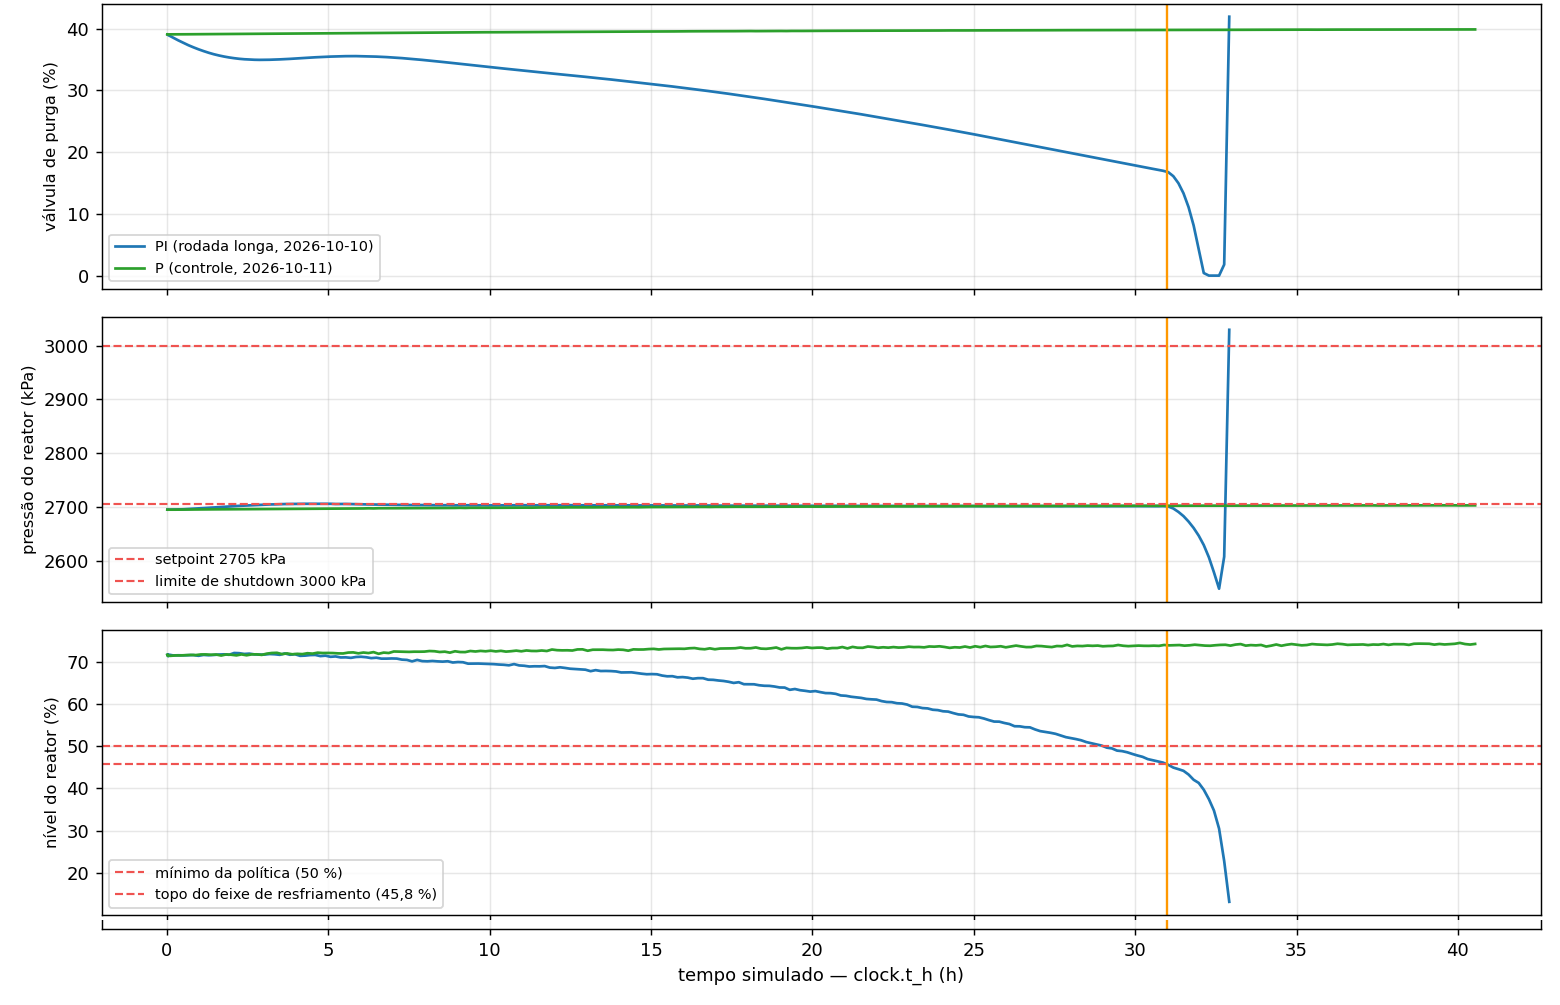
\includegraphics[width=\linewidth]{exp27-purga-pressao-nivel}
\fonte{PI (azul) contra P (verde): com P, a planta converge em 40~h.}
\column{0.43\textwidth}
\vspace{2pt}
\begin{enumerate}\setlength{\itemsep}{3pt}\small
  \item O PI segura a pressão fechando a purga: 39 $\rightarrow$ 18~\% em 30~h
  \item O inerte B se acumula e o nível do reator, \textbf{sem malha}, cai: \mbox{72 $\rightarrow$ 46~\%}
  \item Abaixo de 45,8~\%, o feixe de resfriamento fica descoberto
  \item A temperatura sobe, a purga satura e a pressão passa de 3000~kPa: parada de emergência
\end{enumerate}
\end{columns}
\end{frame}

% ---------------------------------------------------------------------------
\begin{frame}{Experimento 27: o que o supervisor viu}
\marcador{Experimento 27: o que o supervisor viu}
\begin{columns}[T]
\column{0.66\textwidth}
\vspace{4pt}
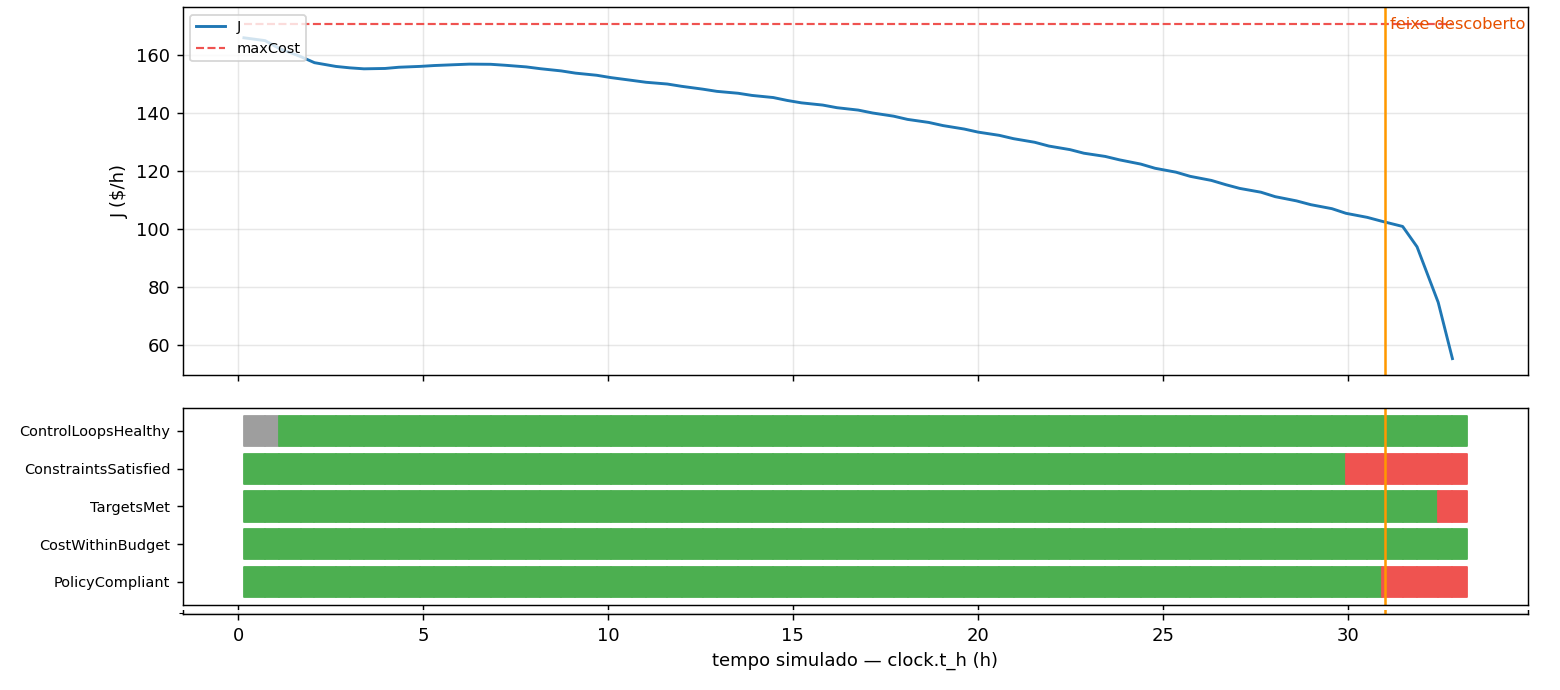
\includegraphics[width=\linewidth]{exp27-custo-conditions}
\fonte{Custo $J$ e \textit{conditions} do supervisor, com as malhas PI.}
\column{0.32\textwidth}
\vspace{2pt}
\begin{itemize}\setlength{\itemsep}{5pt}
  \item $J$ caiu de 166 para 55~\$/h: menos purga, menos reagente perdido
  \item Custo e malhas: \textit{True} até o fim
  \item Só o \textbf{limite de nível} percebeu, em 30,9~h, e tarde
\end{itemize}
\end{columns}
\end{frame}

% ===========================================================================
\begin{frame}{Conclusões}
\marcador[0]{Fechamento}
\marcador[1]{Conclusões}
\vspace{2pt}
\begin{tikzpicture}\node[fill=cinzaClaro,rounded corners=3pt,inner sep=7pt,text width=\linewidth-14pt,align=flush left]{%
\textbf{O objetivo foi atingido.} O Kubernetes observou a planta e julgou a política declarada, sem conhecer o TEP.};\end{tikzpicture}
\par\vspace{2pt}
\begin{minipage}{0.84\textwidth}
\begin{enumerate}\setlength{\itemsep}{4pt}\small
  \item \textbf{O Kubernetes consegue observar e julgar:} \texttt{Compliant} em operação normal e \texttt{NonCompliant} sob o IDV(6), com a política fixa
  \item \textbf{As respostas de P1 a P4 que implementei tiveram problemas:} escala do índice invertida, orçamento calibrado num transitório, malhas PI sem malha de nível
  \item \textbf{O veredito vale o que vale a política:} com critérios errados, o supervisor não vê o que deveria, como no Experimento 27
  \item \textbf{Falta escolher como construir a política:} quais métodos de P1 a P4 dão os melhores critérios
\end{enumerate}
\end{minipage}
\end{frame}

% ---------------------------------------------------------------------------
\begin{frame}{Trabalhos futuros}
\marcador{Trabalhos futuros}
\vspace{6pt}
\begin{columns}[T]
\column{0.48\textwidth}
\caixaFuturo{1. Corrigir os erros}{escala do índice, janelas em tempo simulado, orçamento em regime e malha de nível do reator}
\par\vspace{6pt}
\caixaFuturo{3. Sensores e atuadores}{avaliar os sinais e transformá-los em indicadores de estado, como na iniciação científica}
\column{0.48\textwidth}
\caixaFuturo{2. Observar uma planta real}{uma planta do laboratório de controle do Ifes, com o mesmo supervisor}
\par\vspace{6pt}
\caixaFuturo{4. Otimização em tempo real}{recalcular o ponto de operação com a planta em operação e atualizar a política}
\end{columns}
\end{frame}

% ---------------------------------------------------------------------------
{\fundo{encerramento}\setbeamertemplate{footline}{}
\begin{frame}[plain]
\marcador[1]{Obrigado}
  \begin{tikzpicture}[remember picture,overlay]
    \node[anchor=north,align=center] at ($(current page.north)+(0.15cm,-6.3cm)$) {%
      {\color{verdeEsc}\Large\bfseries Obrigado!}\\[3pt]
      {\color{cinza}\footnotesize Matheus Corteletti Delfino}};
  \end{tikzpicture}
\end{frame}}

% ===========================================================================
% RESERVA: para as perguntas
\setbeamertemplate{footline}{%
  \hspace*{1.6cm}\raisebox{0.32cm}{\scriptsize\color{cinza!70}\insertframenumber\quad\Acrobatmenu{GoBack}{\beamerreturnbutton{Voltar}}\,\hyperlink{ap-indice}{\beamergotobutton{Reserva}}}}
% ---------------------------------------------------------------------------
\begin{frame}[label=ap-indice]{Reserva}
\marcador[0]{Reserva}
\vspace{4pt}
\begin{columns}[T]
\column{0.47\textwidth}
\begin{itemize}\setlength{\itemsep}{4pt}
  \item \hyperlink{ap-fortran}{\textcolor{verdeIF}{Código original em FORTRAN}}
  \item \hyperlink{ap-tep-plant}{\textcolor{verdeIF}{O \texttt{tep-plant} em Rust}}
  \item \hyperlink{ap-modos}{\textcolor{verdeIF}{Modos de operação}}
  \item \hyperlink{ap-disturbios}{\textcolor{verdeIF}{Distúrbios}}
  \item \hyperlink{ap-custo}{\textcolor{verdeIF}{Função de custo}}
  \item \hyperlink{ap-otimo}{\textcolor{verdeIF}{Ponto de operação ótimo}}
\end{itemize}
\column{0.47\textwidth}
\begin{itemize}\setlength{\itemsep}{4pt}
  \item \hyperlink{ap-parcelas}{\textcolor{verdeIF}{Custo por parcela}}
  \item \hyperlink{ap-p-pi}{\textcolor{verdeIF}{Malhas P e PI}}
  \item \hyperlink{ap-preditividade}{\textcolor{verdeIF}{Índice de preditividade}}
  \item \hyperlink{ap-velocidade}{\textcolor{verdeIF}{Velocidade e janelas}}
  \item \hyperlink{ap-containers}{\textcolor{verdeIF}{Containers}}
\end{itemize}
\end{columns}
\end{frame}


% ---------------------------------------------------------------------------
\begin{frame}[label=ap-fortran]{Código original em FORTRAN}
\marcador{Código original em FORTRAN}
\centering
\href{https://github.com/camaramm/tennessee-eastman-profBraatz}{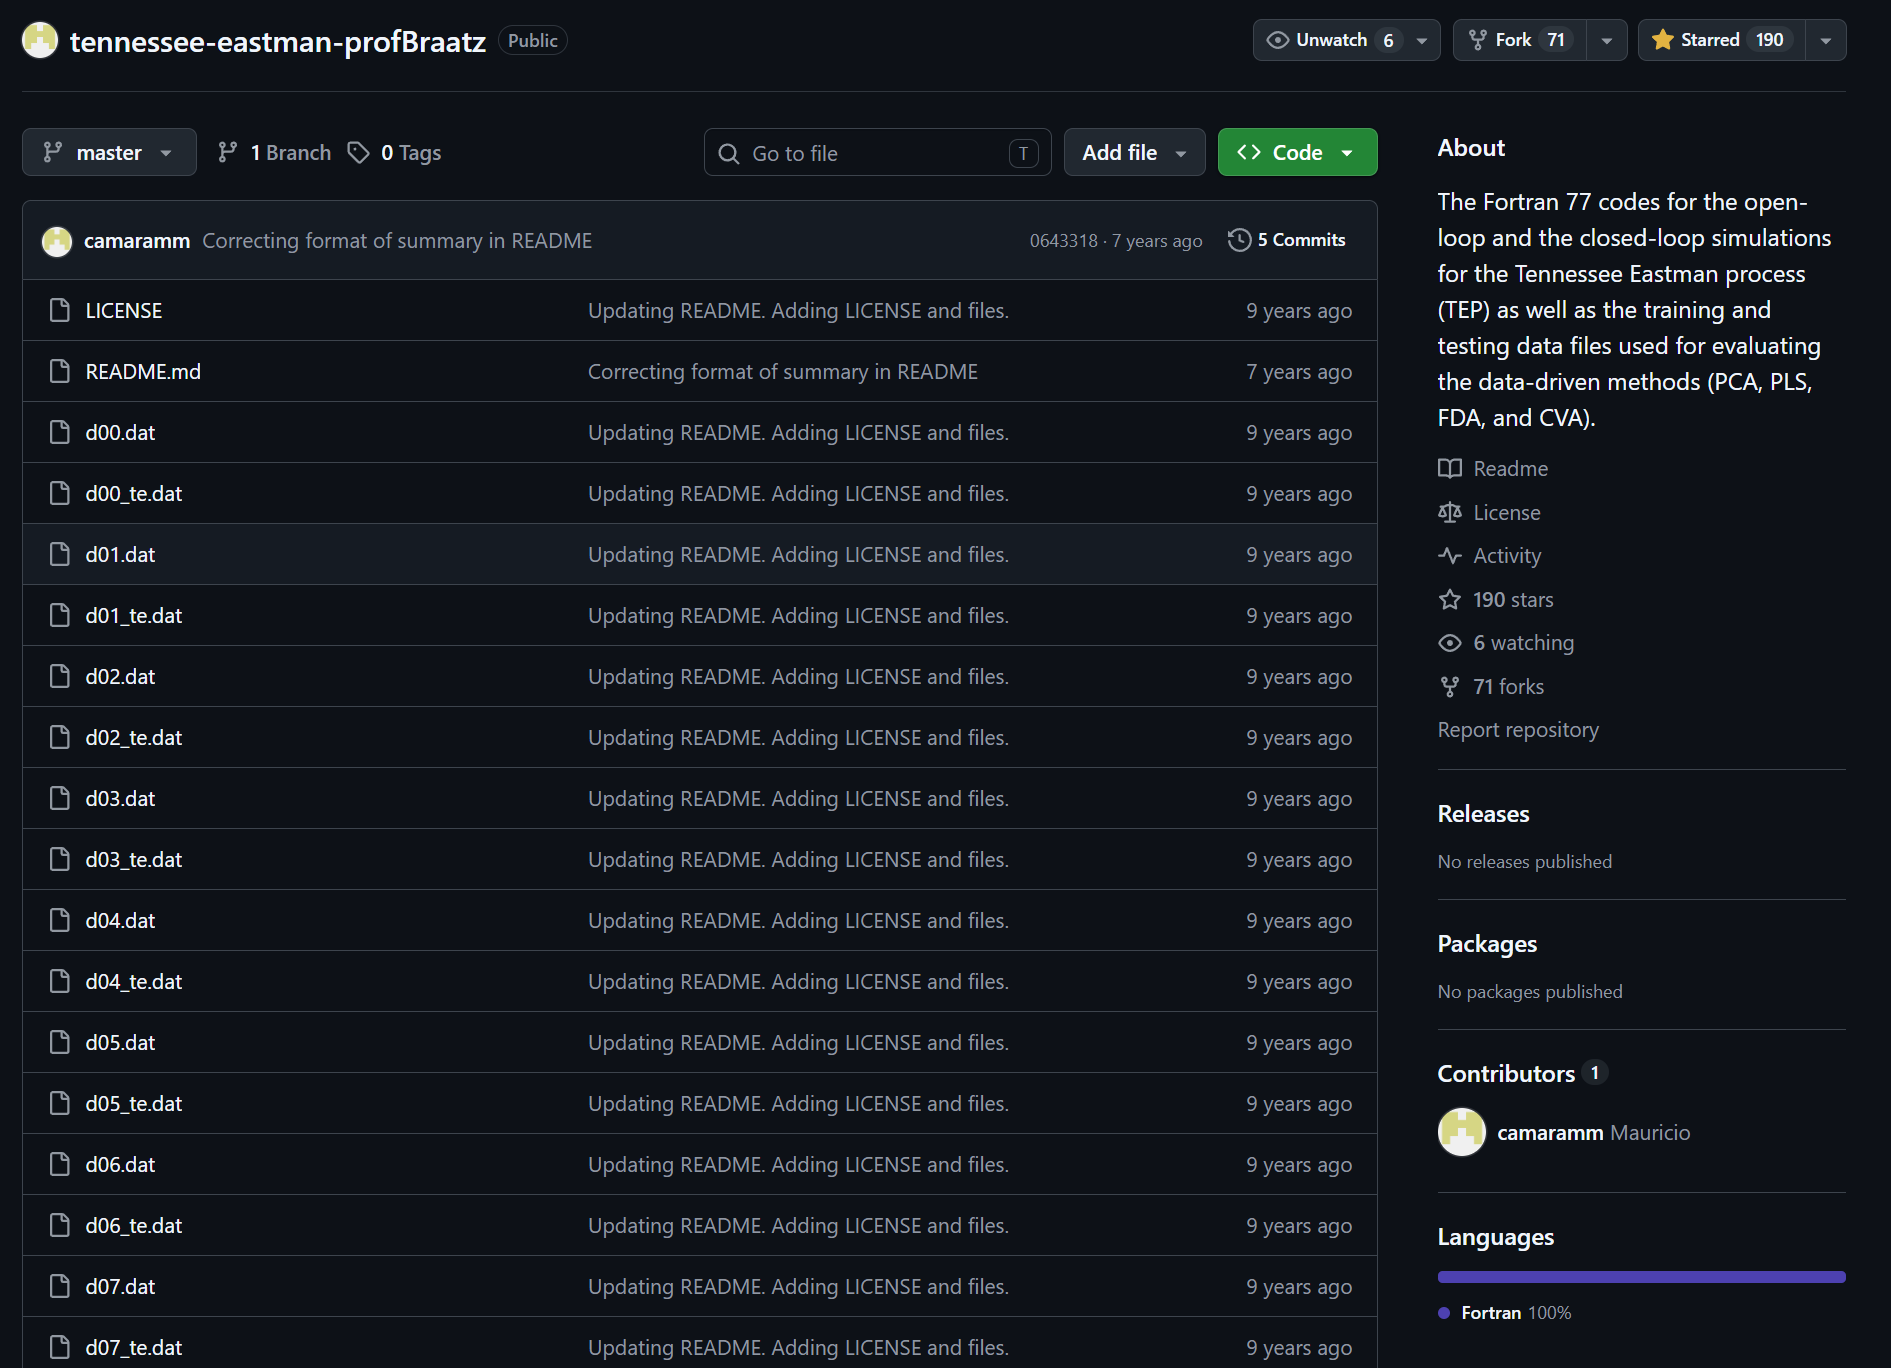
\includegraphics[height=0.72\textheight]{profBraatz-repo-recorte}}
\fonte{\href{https://github.com/camaramm/tennessee-eastman-profBraatz}{\textcolor{verdeIF}{\texttt{github.com/camaramm/tennessee-eastman-profBraatz}}}: versão do grupo de Richard Braatz.}
\end{frame}

% ---------------------------------------------------------------------------
\begin{frame}[label=ap-tep-plant]{O \texttt{tep-plant}: a reescrita em Rust}
\marcador{O tep-plant: a reescrita em Rust}
\centering
\href{https://github.com/Green-Cinnamon-Labs/tep-plant}{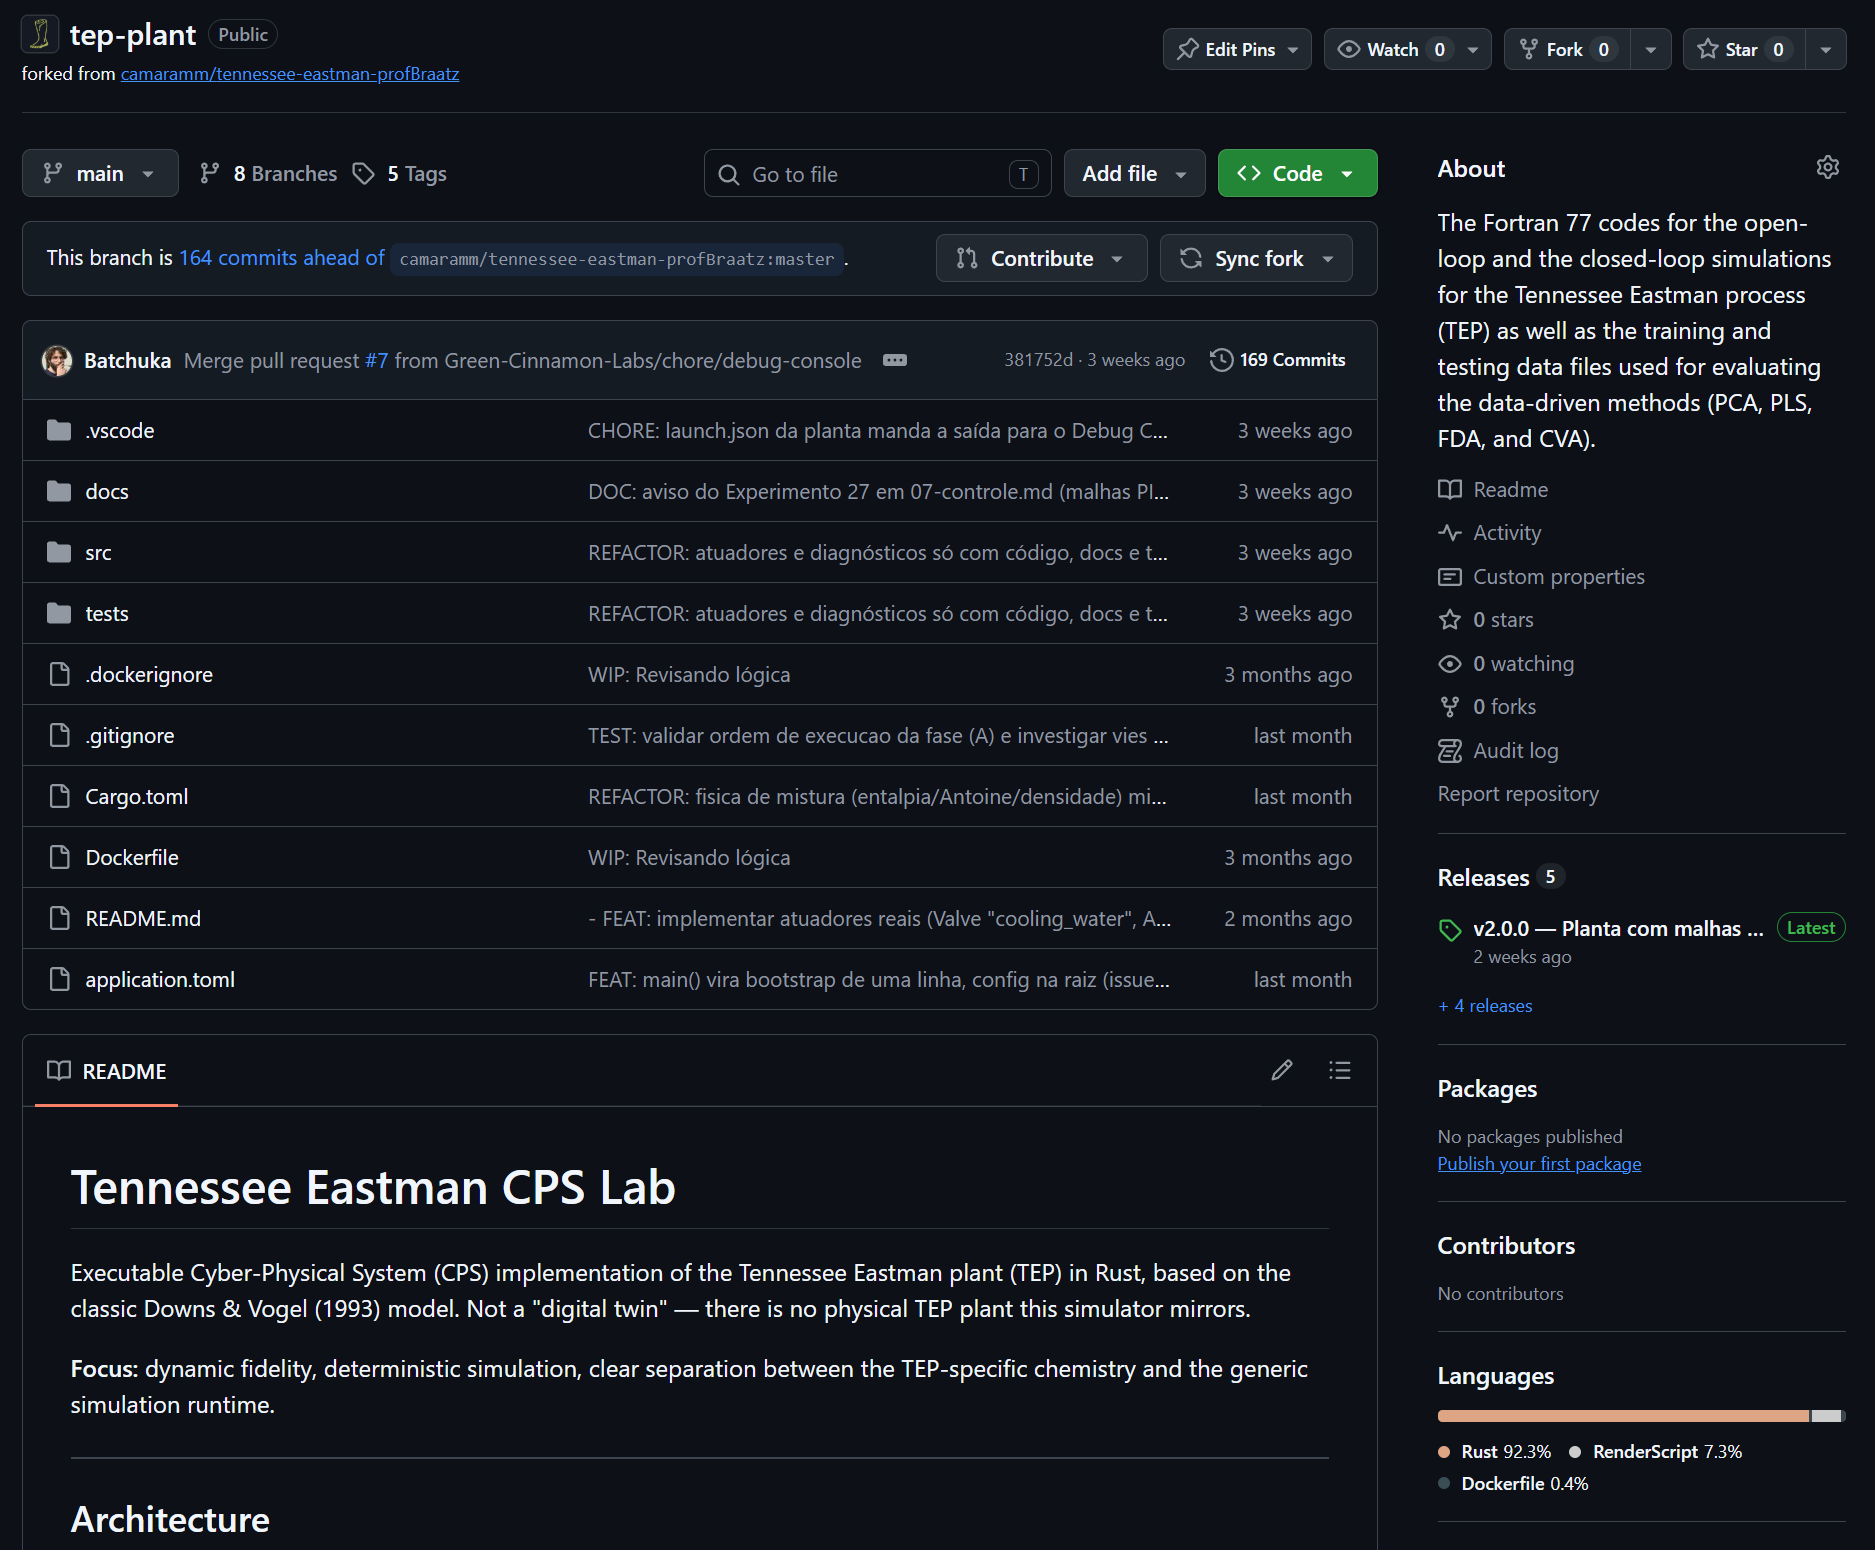
\includegraphics[height=0.72\textheight]{profBraatz-fork-recorte}}
\fonte{\href{https://github.com/Green-Cinnamon-Labs/tep-plant}{\textcolor{verdeIF}{\texttt{github.com/Green-Cinnamon-Labs/tep-plant}}}: fork do original, em Rust.}
\end{frame}

% ---------------------------------------------------------------------------
\begin{frame}[label=ap-modos]{Modos de operação do TEP}
\marcador{Modos de operação do TEP}
\begin{columns}[T]
\column{0.52\textwidth}
\vspace{6pt}
\footnotesize
\begin{tabular}{ccl}
\toprule
\textbf{Modo} & \textbf{G/H (massa)} & \textbf{Produção (kg/h)} \\
\midrule
\textcolor{verdeIF}{\textbf{1}} & \textcolor{verdeIF}{\textbf{50/50}} & \textcolor{verdeIF}{\textbf{7038 G + 7038 H}} \\
2 & 10/90 & 1408 G + 12\,669 H \\
3 & 90/10 & 10\,000 G + 1111 H \\
4 & 50/50 & máxima \\
5 & 10/90 & máxima \\
6 & 90/10 & máxima \\
\bottomrule
\end{tabular}
\fonte{Downs e Vogel (1993). Em verde, o modo usado neste trabalho.}
\column{0.44\textwidth}
\vspace{6pt}
\destaque{\small\textbf{Modo~1}: o caso base\\[2pt]
\scriptsize
Pressão do reator: 2705~kPa\\
Temperatura do reator: 120,4~°C\\
Custo no caso base: 170,6~\$/h\\
Custo no ótimo (Ricker): 114,3~\$/h}
\vspace{4pt}
\destaque{\small\textbf{Limites de operação}\\[2pt]
\scriptsize
Pressão do reator $<$ 2895~kPa\\
Temperatura do reator $<$ 150~°C\\
Parada da planta: pressão $>$ 3000~kPa}
\end{columns}
\end{frame}

% ---------------------------------------------------------------------------
\begin{frame}[label=ap-disturbios]{Distúrbios de Downs e Vogel}
\marcador{Distúrbios de Downs e Vogel}
\begin{columns}[T]
\column{0.45\textwidth}
\vspace{4pt}
\scriptsize
\begin{tabular}{cl}
\toprule
\textbf{IDV} & \textbf{Degraus} \\
\midrule
\textcolor{verdeIF}{\textbf{1}} & \textcolor{verdeIF}{\textbf{razão A/C na alimentação 4}} \\
\textcolor{verdeIF}{\textbf{2}} & \textcolor{verdeIF}{\textbf{teor de B na alimentação 4}} \\
\textcolor{verdeIF}{\textbf{3}} & \textcolor{verdeIF}{\textbf{temperatura da alimentação de D}} \\
4 & temperatura da água do reator \\
5 & temperatura da água do condensador \\
\textcolor{verdeIF}{\textbf{6}} & \textcolor{verdeIF}{\textbf{perda da alimentação de A}} \\
\textcolor{verdeIF}{\textbf{7}} & \textcolor{verdeIF}{\textbf{pressão do cabeçalho de C}} \\
\bottomrule
\end{tabular}
\column{0.52\textwidth}
\vspace{4pt}
\scriptsize
\setlength{\tabcolsep}{4pt}
\begin{tabular}{cll}
\toprule
\textbf{IDV} & \textbf{O que muda} & \textbf{Tipo} \\
\midrule
8 & composição de A, B e C & aleatório \\
9, 10 & temperatura das alim. D e C & aleatório \\
11, 12 & temperatura das águas & aleatório \\
13 & cinética das reações & deriva \\
14, 15 & válvulas das águas & travamento \\
16 a 20 & não informado no artigo & --- \\
\bottomrule
\end{tabular}
\end{columns}
\vspace{12pt}
\begin{minipage}{0.82\textwidth}
\footnotesize
\textcolor{verdeIF}{\textbf{Em verde: implementados no \texttt{tep-plant}.}}
O 4 e o 5 não têm efeito, porque a água de resfriamento é constante nesta versão. Os aleatórios dependem de um gerador de sinal, e os travamentos, de um mecanismo no atuador.
\end{minipage}
\end{frame}

% ---------------------------------------------------------------------------
\begin{frame}[label=ap-custo]{Função de custo de Downs e Vogel}
\marcador{Função de custo de Downs e Vogel}
\vspace{8pt}
\begin{center}\footnotesize
$\displaystyle
J =\underbrace{\Big(\sum_{i} c_i\, x_{i}^{\mathrm{purga}}\Big)\,44{,}79\,F_{\mathrm{purga}}}_{\text{reagente perdido na purga}}
  + \underbrace{\Big(\sum_{i \in \{D,E,F\}} c_i\, x_{i}^{\mathrm{prod}}\Big)\,9{,}21\,F_{\mathrm{prod}}}_{\text{impurezas no produto}}
  + \underbrace{0{,}0536\,W_{\mathrm{comp}}}_{\text{compressor}}
  + \underbrace{0{,}0318\,F_{\mathrm{vapor}}}_{\text{vapor}}$
\end{center}
\begin{center}
\footnotesize
\begin{tabular}{lccccccc}
\toprule
 & A & C & D & E & F & G & H \\
\midrule
$c_i$ (\$/kmol) & 2,206 & 6,177 & 22,06 & 14,56 & 17,89 & 30,44 & 22,94 \\
\bottomrule
\end{tabular}
\end{center}
\vspace{-2pt}
\begin{minipage}{0.82\textwidth}
\begin{itemize}\footnotesize\setlength{\itemsep}{1pt}
  \item B é inerte e não tem custo; G e H só contam quando saem na purga
  \item $F_{\mathrm{purga}}$ em kscmh e $F_{\mathrm{prod}}$ em m³/h; 44,79 e 9,21 convertem para kmol/h
  \item $W_{\mathrm{comp}}$ em kW e $F_{\mathrm{vapor}}$ em kg/h; $x_i$ vem das composições medidas
  \item No supervisor, a mesma conta vira os 12 termos do \texttt{CostFunction}
\end{itemize}
\end{minipage}
\end{frame}

% ---------------------------------------------------------------------------
\begin{frame}[label=ap-otimo]{Ponto de operação ótimo}
\marcador{Ponto de operação ótimo}
\begin{columns}[T]
\column{0.52\textwidth}
\centering
\vspace{14pt}
\begin{tikzpicture}[
    scale=0.66, every node/.style={transform shape},
    font=\small,
    rotulo/.style={font=\scriptsize},
    limite/.style={vermelhoIF}
]
  % escala: x = (P - 2650)/300 * 9 cm; y = (T - 119)/7 * 5,5 cm
  \fill[gray!12] (4.5,0) rectangle (9,5.5);
  \begin{scope}
    \clip (0,0) rectangle (9,5.5);
    \foreach \r in {0.6,1.1,2.3,3.1,3.9}
      \draw[gray!55] (7,3.06) ellipse ({1.6*\r} and {\r});
    \draw[gray!80!black] (7,3.06) ellipse (2.5 and 1.5625);
  \end{scope}
  \draw (0,0) rectangle (9,5.5);
  \foreach \p/\x in {2700/1.5, 2800/4.5, 2900/7.5}
    \draw (\x,0) -- (\x,-0.1) node[below, rotulo] {\p};
  \foreach \t/\y in {120/0.786, 122/2.357, 124/3.929}
    \draw (0,\y) -- (-0.1,\y) node[left, rotulo] {\t};
  \node[below] at (4.5,-0.45) {pressão do reator (kPa)};
  \node[rotate=90, above] at (-0.55,2.75) {temperatura do reator (°C)};
  \draw[limite, very thick] (4.5,0) -- (4.5,5.5);
  \foreach \y in {0.1,0.4,...,5.3}
    \draw[limite] (4.5,\y) -- ++(0.18,0.18);
  \node[above, rotulo, limite, align=center] at (4.5,5.5) {pressão máxima adotada (2800~kPa)};
  \node[rotulo, gray!60!black] at (7.4,0.35) {região inviável};
  \draw[dashed, -{Latex[length=2mm]}, verdeEsc] (1.72,1.15) -- (4.38,2.98);
  \draw[thick, fill=white] (1.65,1.1) circle (0.09);
  \node[below right, rotulo, align=left, fill=white, inner sep=1pt] at (1.7,1.0) {caso base\\$J = 170{,}6$~\$/h};
  \fill[verdeEsc] (4.5,3.06) circle (0.1);
  \node[above left, rotulo, align=right, text=verdeEsc, fill=white, inner sep=1pt] at (4.4,3.15) {ótimo do Modo~1\\$J \approx 114{,}3$~\$/h};
  \draw (7,3.06) circle (0.1);
  \fill (7,3.06) circle (0.03);
  \node[below, rotulo, align=center, fill=gray!12, inner sep=1pt] at (7,2.9) {menor $J$\\sem o limite};
  \node[right, rotulo, fill=white, inner sep=1pt] at (0.15,5.0) {curvas de mesmo $J$};
\end{tikzpicture}
\fonte{Esquema com 2 dos 8 graus de liberdade (Ricker, 1995).}
\column{0.45\textwidth}
\vspace{2pt}
\begin{itemize}\setlength{\itemsep}{4pt}
  \item Entre os pontos que cumprem o modo e os limites, o de menor $J$, em regime
  \item 8 graus de liberdade; Ricker (1995) resolveu com o modelo completo
  \item 5 variáveis encostam num limite, como a pressão em 2800~kPa; as outras 3 ficam num mínimo dentro da faixa
  \item $J$: 170,6 $\rightarrow$ 114,3~\$/h, com menos perda na purga
\end{itemize}
\end{columns}
\end{frame}

\begin{frame}[label=ap-parcelas]{Custo no caso base, por parcela}
\marcador{Custo no caso base, por parcela}
\centering\vspace{6pt}
\begin{tabular}{lcc}
\toprule
\textbf{Parcela (\$/h)} & \textbf{Planta} & \textbf{Ricker (1995)} \\
\midrule
Purga & 114,730 & 114,71 \\
Produto & 30,271 & 30,28 \\
Compressor & 18,301 & 18,30 \\
Vapor & 7,324 & 7,32 \\
\midrule
\textbf{Total} & \textbf{170,626} & \textbf{170,61} \\
\bottomrule
\end{tabular}\par
\vspace{12pt}
\begin{minipage}{0.80\textwidth}
\begin{itemize}
  \item Planta avaliada como função (modo função do monjolo), sem tempo e sem controle
  \item Diferenças conhecidas: água de resfriamento constante nas versões com o supervisor, analisadores contínuos e distúrbios aleatórios ainda não implementados
\end{itemize}
\end{minipage}
\end{frame}

\begin{frame}[label=ap-p-pi]{Malhas P e PI na pressão do reator}
\marcador{Malhas P e PI na pressão do reator}
\vspace{4pt}
\begin{columns}[T]
\column{0.48\textwidth}
\destaque{\textbf{Malha P na pressão}\\[2pt]\footnotesize
A pressão pode parar alguns kPa fora do \textit{setpoint}. Essa folga deixa a planta se ajustar: o nível do reator sobe um pouco, e tudo para.}
\column{0.48\textwidth}
\destaque{\textbf{Malha PI na pressão}\\[2pt]\footnotesize
A pressão fica presa no \textit{setpoint}. Quem absorve o desbalanço é a purga, que decide quanto gás sai, mas não quanto líquido fica no reator.}
\end{columns}
\vspace{10pt}
\begin{minipage}{0.86\textwidth}
\small Isto é uma leitura dos dados, não algo provado. O que está provado: mesma planta, mesmo ruído e mesma velocidade; com P converge e com PI diverge. O teste direto, com PI só nos níveis, ficou pendente.
\end{minipage}
\end{frame}

% ---------------------------------------------------------------------------
\begin{frame}[label=ap-preditividade]{Índice de preditividade: o erro que pode ser previsto}
\marcador{Índice de preditividade: o erro que pode ser previsto}
\centering
\vspace{10pt}
\begin{tikzpicture}[scale=0.86, every node/.style={transform shape},
    font=\small,
    rotulo/.style={font=\scriptsize},
    medido/.style={cinza, thick},
    previsto/.style={verdeIF, thick, dashed},
    caixa/.style={draw=gray!50, fill=cinzaClaro, rounded corners=2pt, minimum width=3.1cm, minimum height=1.0cm, align=center, font=\scriptsize, text=cinza},
    fluxo/.style={-{Latex[length=2mm]}, thick, gray!60}
]
  % ---------- erro com padrão previsível ----------
  \begin{scope}
    \node[anchor=south, text=cinza] at (3.3,1.25) {erro com padrão previsível: \textbf{PI baixo}};
    \draw[-{Latex[length=2mm]}, gray!70] (0,0) -- (6.6,0);
    \node[rotulo, anchor=north east, text=cinza] at (6.6,-1.05) {tempo};
    \draw[gray!70] (0,-1.1) -- (0,1.1);
    \node[rotulo, rotate=90, above, text=cinza] at (0,0) {erro};
    \draw[medido] plot[domain=0.1:6.3, samples=90, smooth] (\x, {0.6*sin(1.8*\x r) + 0.25*sin(0.6*\x r)});
    \draw[previsto] plot[domain=0.6:6.3, samples=90, smooth] (\x, {0.55*sin(1.8*\x r - 0.18) + 0.25*sin(0.6*\x r)});
  \end{scope}

  % ---------- erro sem padrão ----------
  \begin{scope}[xshift=7.8cm]
    \node[anchor=south, text=cinza] at (3.3,1.25) {erro sem padrão, como ruído: \textbf{PI perto de 1}};
    \draw[-{Latex[length=2mm]}, gray!70] (0,0) -- (6.6,0);
    \node[rotulo, anchor=north east, text=cinza] at (6.6,-1.05) {tempo};
    \draw[gray!70] (0,-1.1) -- (0,1.1);
    \pgfmathsetseed{11}
    \draw[medido] plot[domain=0.1:6.3, samples=60] (\x, {0.75*rand});
    \draw[previsto] plot[domain=0.6:6.3, samples=40, smooth] (\x, {0.08*sin(2.2*\x r)});
  \end{scope}

  % legenda
  \draw[medido] (3.6,-1.8) -- (4.2,-1.8);
  \node[rotulo, right, text=cinza] at (4.2,-1.8) {erro medido};
  \draw[previsto] (6.6,-1.8) -- (7.2,-1.8);
  \node[rotulo, right, text=cinza] at (7.2,-1.8) {erro previsto a partir do passado};

  % ---------- triagem diária ----------
  \node[caixa] (c1) at (1.55,-2.8)  {3000 malhas PID\\analisadas toda noite};
  \node[caixa] (c2) at (5.55,-2.8)  {PI de cada malha\\em janelas de tempo};
  \node[caixa] (c3) at (9.55,-2.8)  {filtros: atuador se move\\e PI baixo persiste};
  \node[caixa] (c4) at (13.55,-2.8) {relatório da manhã: cerca\\de 150 malhas sinalizadas};
  \draw[fluxo] (c1) -- (c2);
  \draw[fluxo] (c2) -- (c3);
  \draw[fluxo] (c3) -- (c4);
\end{tikzpicture}
\fonte{Elaborado pelo autor, com base em Bradu \textit{et al.} (2018). Sinais ilustrativos. Figura do Cap. 2 da monografia.}
\end{frame}

\begin{frame}[label=ap-velocidade]{Velocidade da simulação e janelas do supervisor}
\marcador{Velocidade da simulação e janelas do supervisor}
\begin{minipage}{0.86\textwidth}
\begin{itemize}\setlength{\itemsep}{6pt}
  \item A física avança sempre 1~s de processo por passo; a velocidade só muda quantos passos por segundo de relógio
  \item As janelas do supervisor e do \textit{historian} são medidas em \textbf{tempo de relógio}
  \item Velocidade 5 ($\approx 10\times$): cada avaliação cobre \textasciitilde5~min de processo
  \item Velocidade 30 ($\approx 56\times$): cada avaliação cobre \textasciitilde28~min, e a janela de 300~s do índice, \textasciitilde4,7~h
  \item Por isso, rodadas em velocidades diferentes não se comparam direto. A correção é medir as janelas pelo sinal \texttt{clock.t\_h}, que a planta já publica
\end{itemize}
\end{minipage}
\end{frame}

\begin{frame}[label=ap-containers]{O laboratório num computador pessoal}
\marcador{O laboratório num computador pessoal}
\centering
\includegraphics[width=0.72\textwidth]{containers-rodando-docker}
\fonte{Três \textit{containers} no Docker Compose (planta, \textit{historian}, IHM) e o nó do Kind.\\Cerca de 1~GB de memória no total; a planta usa 15~MB.}
\end{frame}

\end{document}
